\documentclass[
%draft%     uncomment to activate draft mode (see preamble/proofs)
]{article}   

% preamble -- do not rearrange order of \includes
%\include{classoptions}
%\include{pagesize}
%\include{packages}
%\include{encoding}         
%\include{fonts}
%\include{ToC}
%\include{contributor}
%\include{copyright}
%\include{bibtex}
%\include{environments}
%\include{sectionoptions}
%\include{headerfooter}
%\include{footnoteformat}
%\include{codesnipets}
%\include{proofs}
\usepackage{amsmath} % for align
\usepackage{subcaption}
\captionsetup{compatibility=false}
\usepackage{algorithm}% http://ctan.org/pkg/algorithms
\usepackage{algpseudocode}% http://ctan.org/pkg/algorithmicx
\usepackage[style=numeric,sorting=none]{biblatex}
\addbibresource{main.bib} %Import the bibliography file
\usepackage{tikz}
\usepackage{graphicx}
\usepackage[export]{adjustbox}
\usepackage{caption}
\usepackage{amssymb}
\usepackage{float}
% \usepackage{subfig}
\usepackage{placeins}
\usepackage{listings}
\lstset{
  basicstyle=\ttfamily,
  mathescape
}
%\usepackage{minted}
\usetikzlibrary{shapes}
\usetikzlibrary {positioning}
\usetikzlibrary{chains}
\usetikzlibrary{fit}
\usetikzlibrary{chains,shadows.blur}
\usepackage{geometry}
\usepackage{array}
\usepackage{hyperref}
\usepackage{indentfirst}
\usepackage{pdfpages}


\hypersetup{
    colorlinks=true,
    linkcolor=magenta,
    filecolor=cyan,      
    urlcolor=blue,
}
\graphicspath{ {./images/} }


\usepackage{listings}
\usepackage{xcolor}

\usepackage[autosize]{dot2texi}
\usepackage{tikz}
\usetikzlibrary{shapes,arrows}

\definecolor{codegreen}{rgb}{0,0.6,0}
\definecolor{codegray}{rgb}{0.5,0.5,0.5}
\definecolor{codepurple}{rgb}{0.58,0,0.82}
\definecolor{backcolour}{rgb}{0.95,0.95,0.92}
\usepackage{tcolorbox}

\newtcolorbox{note}[1]{colback=red!5!white,colframe=red!75!black,fonttitle=\bfseries,title=#1}


\newtcolorbox{definition}[1]{colback=blue!5!white,colframe=blue!75!black,fonttitle=\bfseries,title=#1}

\lstdefinestyle{mystyle}{
    % backgroundcolor=\color{backcolour},   
    commentstyle=\color{codegreen},
    keywordstyle=\color{magenta},
    numberstyle=\tiny\color{codegray},
    stringstyle=\color{codepurple},
    basicstyle=\ttfamily\footnotesize,
    breakatwhitespace=false,         
    breaklines=true,                 
    captionpos=b,                    
    keepspaces=true,                 
    numbers=left,                    
    numbersep=5pt,                  
    showspaces=false,                
    showstringspaces=false,
    showtabs=false,                  
    tabsize=2
}

\newtcolorbox{proof}[1]{colback=white,colframe=gray,fonttitle=\bfseries,title=#1}


% \lstset{style=mystyle}


  \lstset{ %
    language=Octave,                % the language of the code
    basicstyle=\footnotesize,           % the size of the fonts that are used for the code
    numbers=left,                   % where to put the line-numbers
    numberstyle=\tiny\color{gray},  % the style that is used for the line-numbers
    stepnumber=2,                   % the step between two line-numbers. If it's 1, each line 
                                    % will be numbered
    numbersep=5pt,                  % how far the line-numbers are from the code
    backgroundcolor=\color{white},      % choose the background color. You must add \usepackage{color}
    showspaces=false,               % show spaces adding particular underscores
    showstringspaces=false,         % underline spaces within strings
    showtabs=false,                 % show tabs within strings adding particular underscores
    frame=single,                   % adds a frame around the code
    rulecolor=\color{black},        % if not set, the frame-color may be changed on line-breaks within not-black text (e.g. commens (green here))
    tabsize=2,                      % sets default tabsize to 2 spaces
    captionpos=b,                   % sets the caption-position to bottom
    breaklines=true,                % sets automatic line breaking
    breakatwhitespace=false,        % sets if automatic breaks should only happen at whitespace
    title=\lstname,                 % show the filename of files included with \lstinputlisting;
                                    % also try caption instead of title
    keywordstyle=\color{blue},          % keyword style
    commentstyle=\color{dkgreen},       % comment style
    stringstyle=\color{mauve},         % string literal style
    escapeinside={\%*}{*)},            % if you want to add LaTeX within your code
    morekeywords={*,...}               % if you want to add more keywords to the set
}


% define issue details
\title{Compiler Optimization Notes}
\newcommand\thejournalsubtitle{Notes for the Compiler Optimization Techniques}
\newcommand\thevolume{}
\newcommand\theseason{May}
\newcommand\theyear{2022}
\newcommand\theissue{\thejournal \ \thevolume \ (\theyear)} 

\newcommand\generaleditor{}
\newcommand\associateeditor{}
\sloppy
\newcommand\thewebsite{https://github.com/liusy58/CompilerNotes}

\begin{document}
\sloppy                         % preferences more space between words over overrunning margins
\lefthyphenmin=3                % suppresses hyphenation after only 1 or 2 characters
                                % NB: You will need to repeat \lefthyphenmin in the text if you use \selectlanguage
%\include{editorialboard}
%\include{titlepage}
%\include{colofon}
\pagenumbering{roman}           
%\tableofcontents  
\thispagestyle{empty}

\maketitle
\tableofcontents

% \include{essays/preface}
\pagenumbering{arabic}


% 
\section{Foundations of Data Flow Analysis}


$\leq$ means more conservative, but not means subset.


\subsection{Transfer Functions}





\subsubsection{monotonicity}

% \begin{tcolorbox}
% efjer
% \end{tcolorbox}

\begin{note}{Monotone framework doesn't mean $ f(x) \leq x$}
For example, reaching definition for just one definition \texttt{a=1} in a BasicBlock(\texttt{BB1}).  \[IN(BB1) = \{\} = x = \top , OUT(BB1) = {a} = f(x) \]
However, $x = \top \leq  f(x)$
\end{note}

\subsubsection{Distributivity}

Not a requirement.

\begin{definition}{Distributivity}

A framework $F,V, \wedge$ is \emph{distributive} is and only if 

\[f(x \wedge y)=f(x) \wedge f(y)\]

which means applying $f$ to the merge input is equal to applying $f$ individually then merge result. 
\end{definition}

Reaching definition is distributive.


Constant Propagation is not distributive. 
\begin{figure}[h]
    \centering
    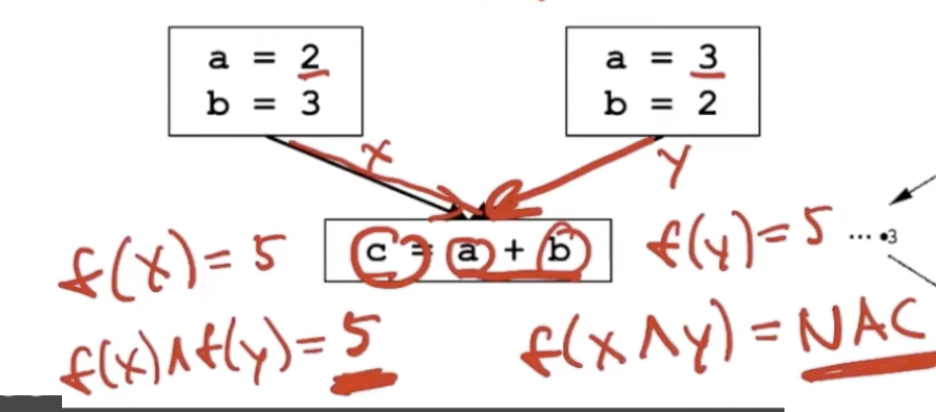
\includegraphics[width=0.2\textwidth]{CDp.png}
    \caption{}
    \label{fig:p15}
\end{figure}

\subsection{Data Flow Analysis}

\begin{definition}{Definition}
Let $f_1, \dots , f_m \in F$, where $f_i$ is the transfer function for node $i$. $f_p=f_{n_k} \cdot \ldots \cdot f_{n_1}$, where $p$ is a path through nodes $n_1  \cdot \ldots \cdot n_k$. $f_p =$ identify function, if $p$ is an empty path.
\end{definition}

\subsubsection{Precision}

Ideally for each node n, the IN should be $ \wedge f_{p_i}(\top)$ for all possibly executed path $p_i$ reaching n. But determining all possible executed paths is undecidable. Look at the example shown in \ref{fig:p20}.


\begin{figure}[h]
    \centering
    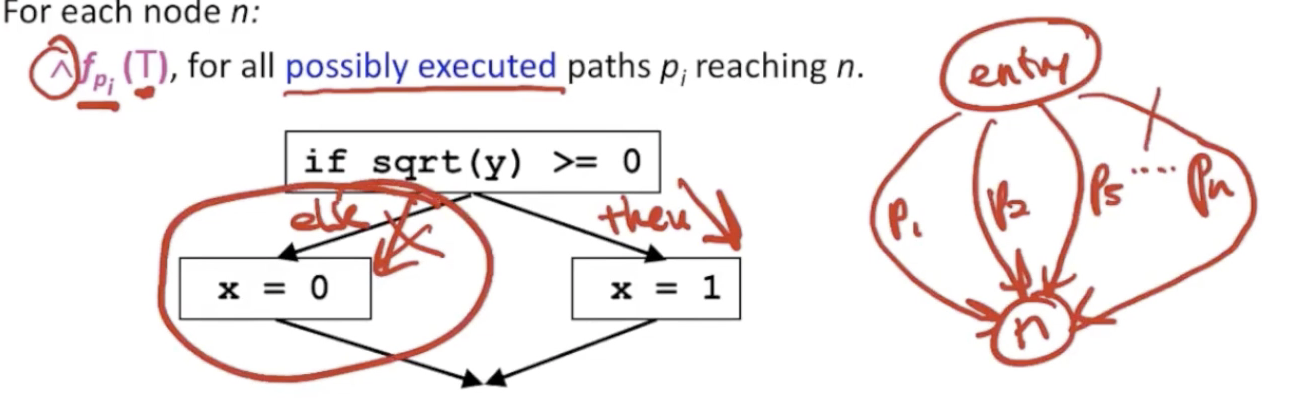
\includegraphics[width=0.2\textwidth]{p20.png}
    \caption{}
    \label{fig:p20}
\end{figure}

So in reality,  we will conservatively include some paths that will never be executed. From a correctness standpoint, this is fine because we will just get an more conservative answer.

\subsubsection{Meet-Over-Path(MOP)}

\begin{definition}{MOP}
For each node n, MOP(n) = $ \wedge f_{p_i}(\top)$ for all possibly executed path $p_i$ reaching n. 

Strictly speaking, MOP considers more paths than necessary, which means 

\[ \textit{MOP = Perfect-Solution} \wedge  \textit{Solution-to-Unexecuted-Paths.}\]

So 

\[ MOP \leq \textit{ Perfect-Solution} \]

MOP is more conservative. 

\end{definition}



\subsection{Solving Data Flow Equations}

Any solution that satisfies equations is a Fixed Point Solution(FP).


\subsubsection{Iterative algorithm }

If framework is monotone and algorithm coverges, then it computes Maximum Fixed Point(MFP).


FP $\leq$ MFP $\leq$ MOP $\leq$ Perfect-solution


Reaching Definition example:
\begin{figure}[h]
    \centering
    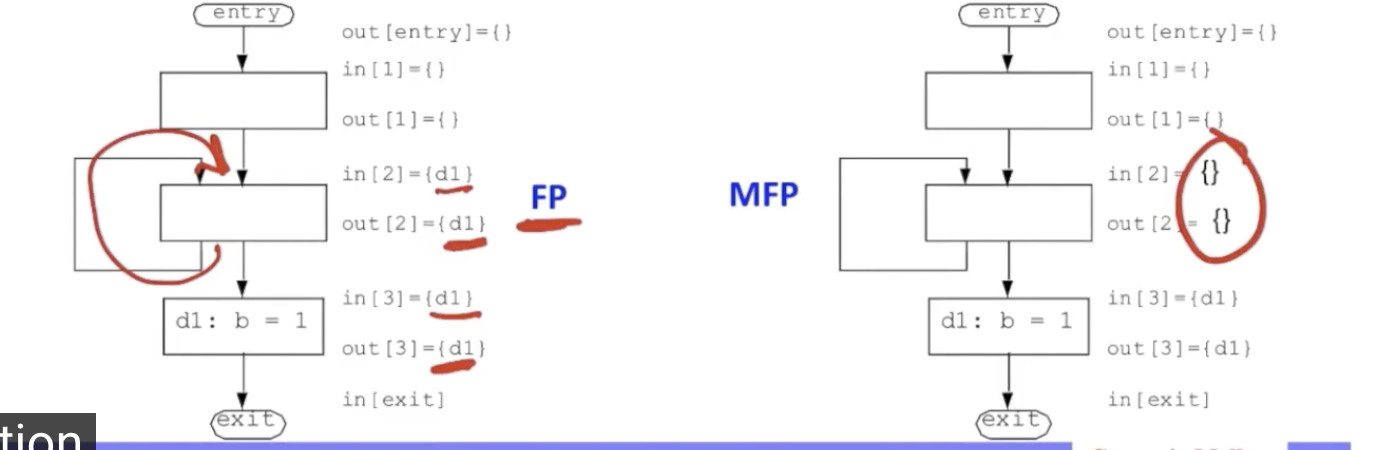
\includegraphics[width=0.2\textwidth]{p21.png}
    \caption{}
    \label{fig:p21}
\end{figure}




\subsection{Precision}

If data flow framework is distributive, then if the algorithm converges, $IN[b] = MOP[b]$

A Monotone but not distributive example: Constant Propagation.(Behaves as if there are additional paths)



\subsection{Convergence}
Properties are needed to guarantee convergence:

\begin{itemize}
    \item monotone
    \item finite descending chain
\end{itemize}



\subsection{Speed of Convergence}

\subsubsection{Reverse Post order}

\begin{figure}[h]
    \centering
    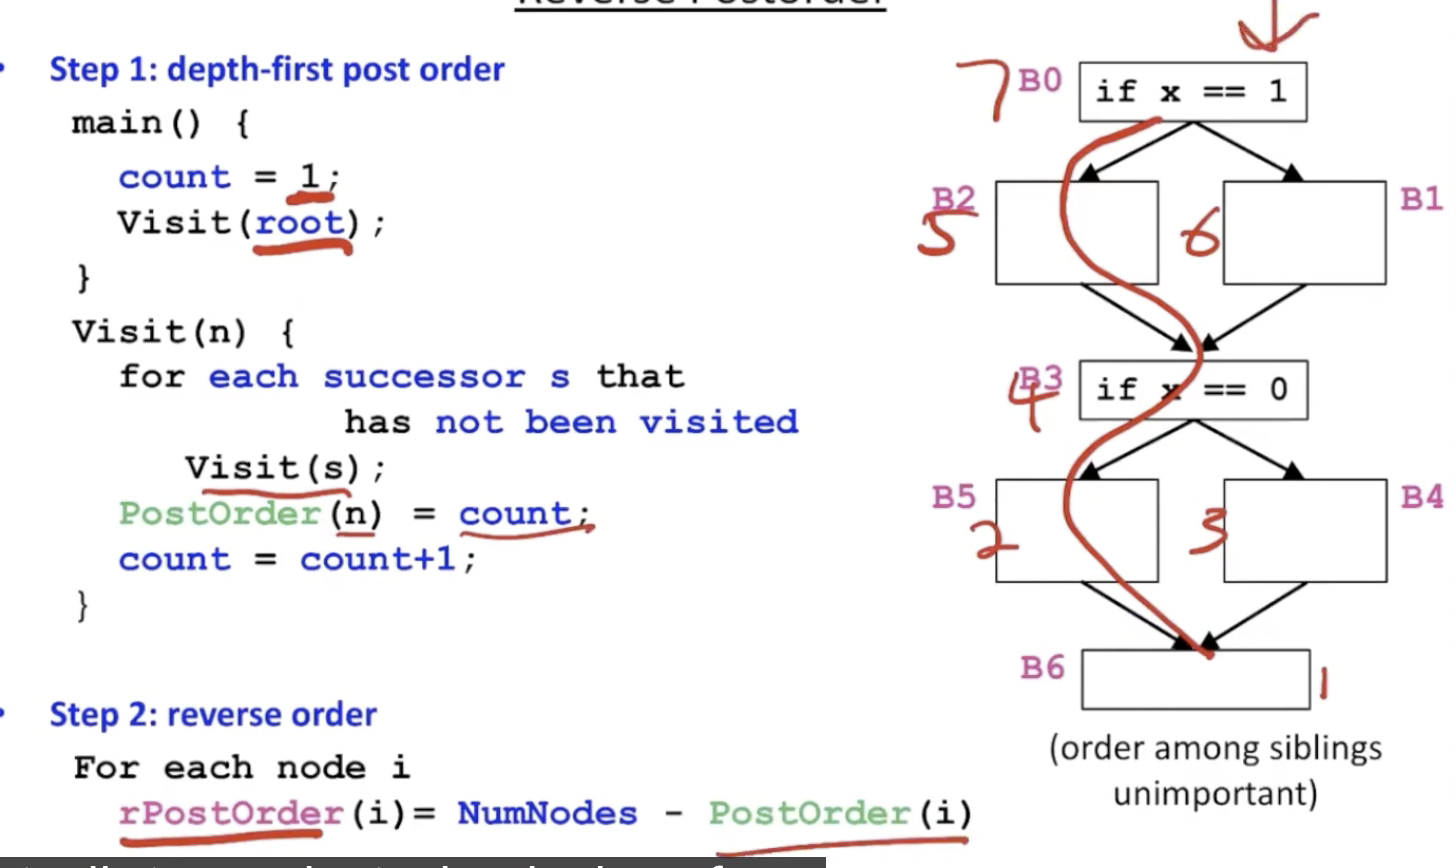
\includegraphics[width=0.2\textwidth]{p22.png}
    \caption{}
    \label{fig:p22}
\end{figure}


\subsubsection{Depth-First Iterative Algorithm(forward)
}



\begin{figure}[h]
    \centering
    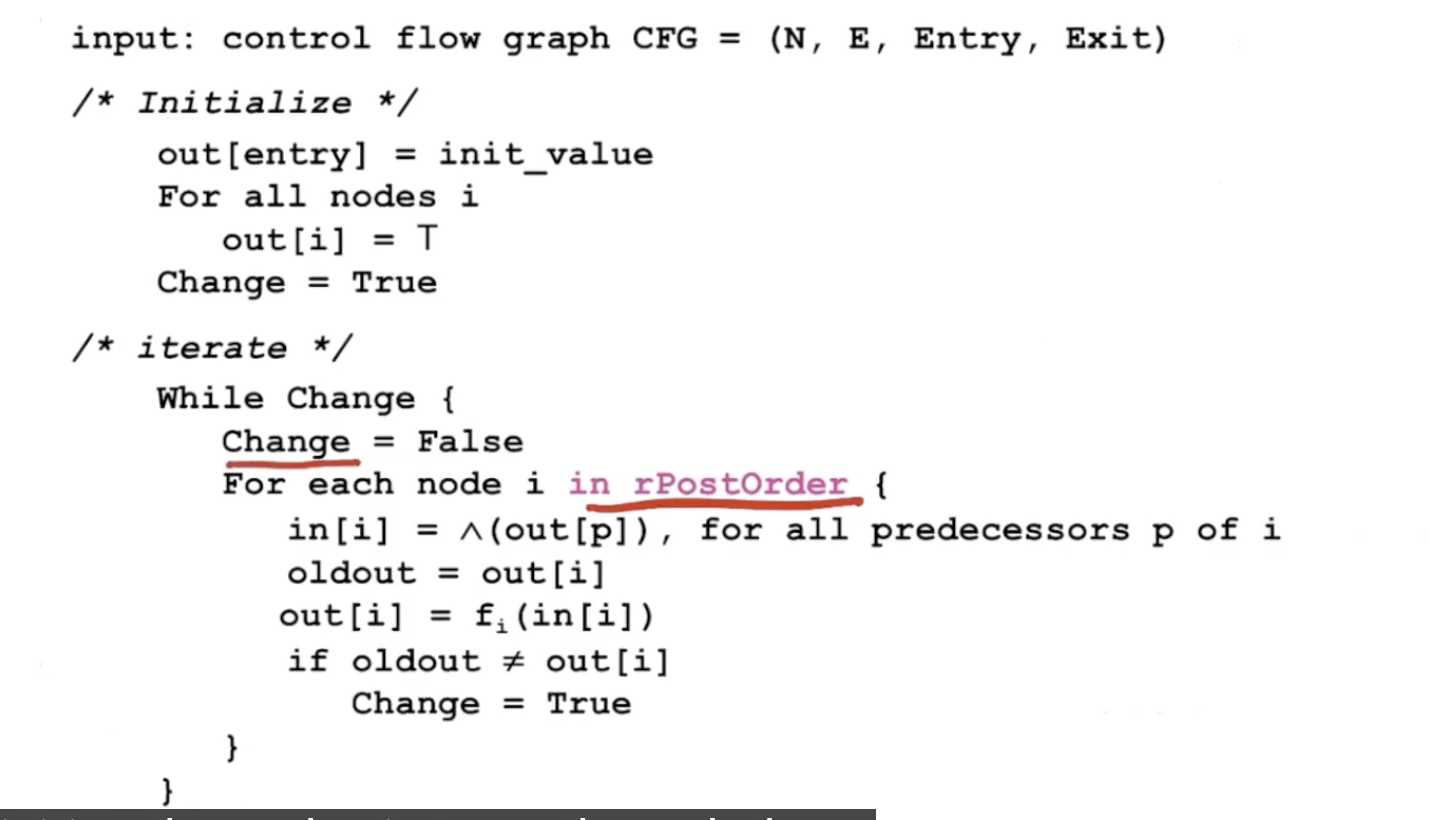
\includegraphics[width=0.2\textwidth]{p23.png}
    \caption{}
    \label{fig:p23}
\end{figure}


\subsubsection{Cost}

Number of iterations = number of back edges in any acyclic path +2 





% \section{More Examples of Data Flow Analysis: Global Common Sub-expression Elimination; Constant Propagation/Folding}

If we care about the past, what happened before, then it is a forward problem (entry). 


\subsection{Available Expression Analysis}


\begin{definition}{Availability of an Expression E at point P}
E is available at P if every path to P in the flow graph
\begin{itemize}
    \item E must be calculated at least once
    \item no variable in E redefined after the last evaluation

\end{itemize}
\end{definition}


\begin{figure}[h]
    \centering
    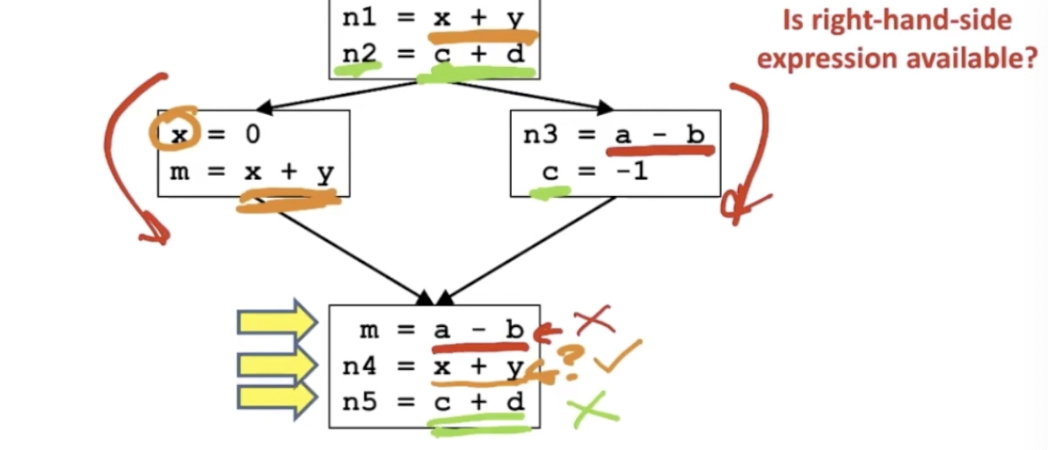
\includegraphics[width=0.3\textwidth]{p24.png}
    \caption{}
    \label{fig:p24}
\end{figure}


\subsubsection{Examples}



In \ref{fig:p24} $a-b$, $c+d$ is not available at the last BB. But $x+y$ is.


\begin{figure}[h]
    \centering
    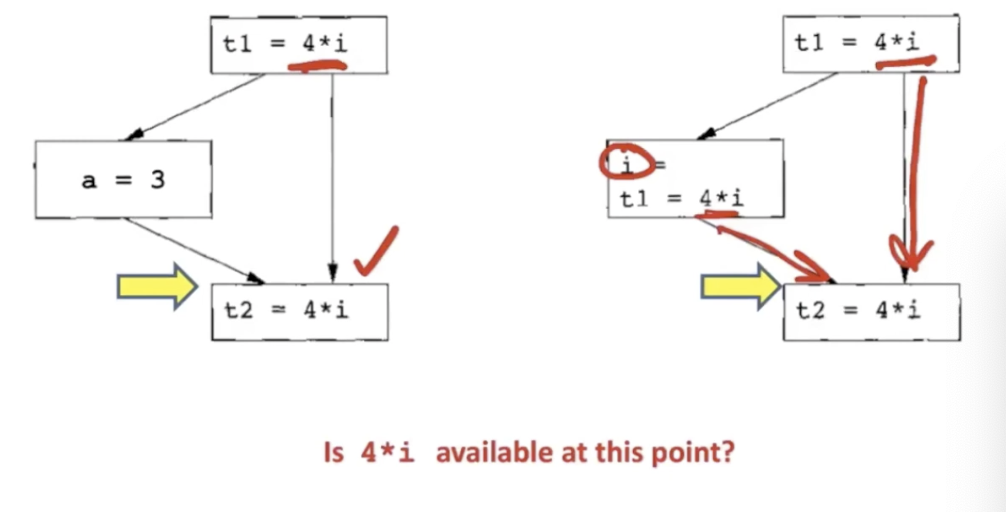
\includegraphics[width=0.3\textwidth]{p25.png}
    \caption{}
    \label{fig:p25}
\end{figure}


In \ref{fig:p25} , $4*i$ is available for both cases.



\begin{figure}[h]
    \centering
    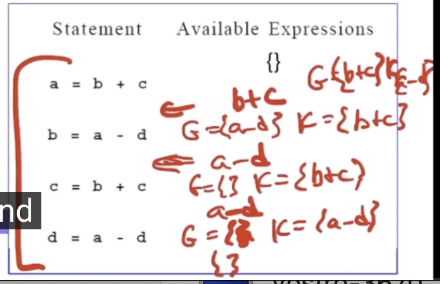
\includegraphics[width=0.3\textwidth]{p26.png}
    \caption{}
    \label{fig:p26}
\end{figure}


In \ref{fig:p26}, we show that calculate transfer functions for complete basic blocks by composing individual instruction transfer functions.


\begin{figure}[h]
    \centering
    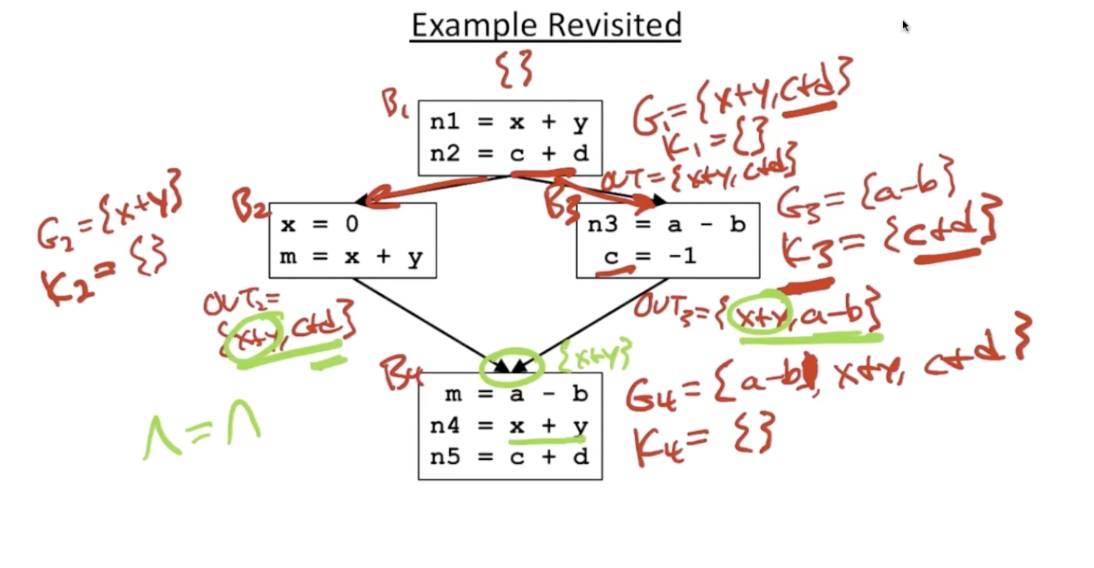
\includegraphics[width=0.3\textwidth]{p27.png}
    \caption{}
    \label{fig:p27}
\end{figure}


\subsection{Eliminating CSEs}


\begin{itemize}
    \item Step1: Value Numbering
    \item Step2: Available expression
    \item Step3: If CSE is an "available expression", then transform the code.
    
\end{itemize}

\begin{figure}[h]
    \centering
    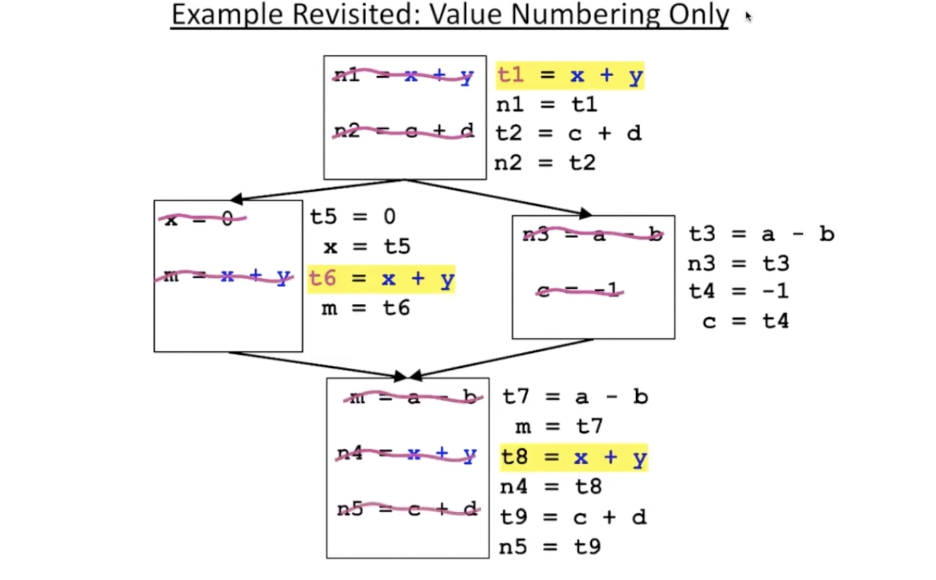
\includegraphics[width=0.3\textwidth]{p28.png}
    \caption{}
    \label{fig:p28}
\end{figure}

If we only use value numbering to eliminate common expression in \ref{fig:p28}, we will see that this will just add a lot of new work and no income. But if we calculate Available expression in \ref{fig:p29}, we can find that $x+y$ is such one and can do some optimization.


\begin{figure}[h]
    \centering
    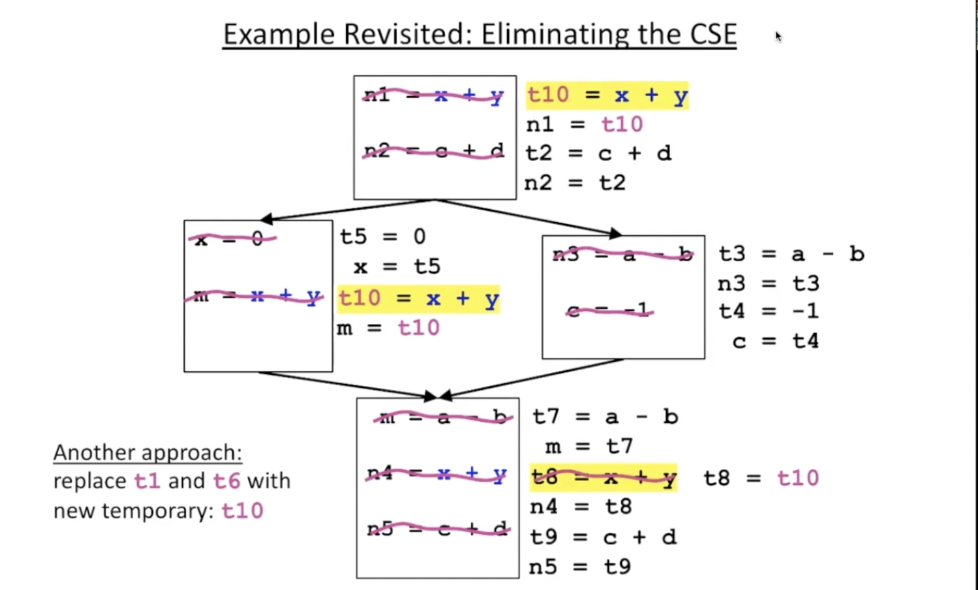
\includegraphics[width=0.3\textwidth]{p29.png}
    \caption{}
    \label{fig:p29}
\end{figure}

\begin{note}{How to deal with Textually identical expression?\ref{fig:p30}}
Just sort the operands.



But for textually different expressions that may be equivalent \ref{fig:p31}, we had better do copy propagation first.

\end{note}
\begin{figure}[h]
    \centering
    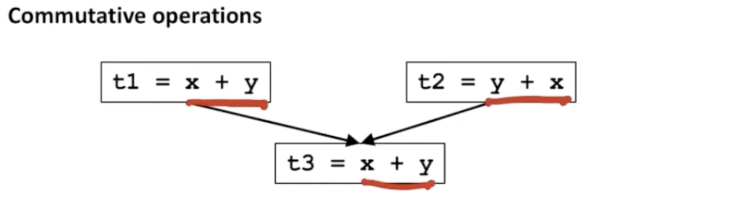
\includegraphics[width=0.3\textwidth]{p30.png}
    \caption{}
    \label{fig:p30}
\end{figure}

\begin{figure}[h]
    \centering
    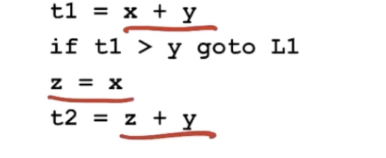
\includegraphics[width=0.3\textwidth]{p31.png}
    \caption{}
    \label{fig:p31}
\end{figure}


\subsubsection{Summary}

\begin{figure}[h]
    \centering
    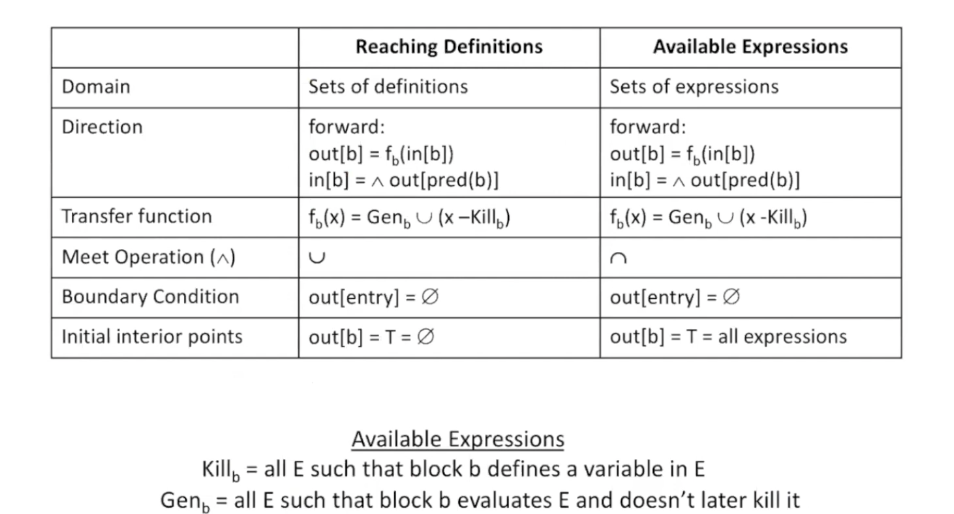
\includegraphics[width=0.3\textwidth]{p32.png}
    \caption{}
    \label{fig:p32}
\end{figure}


\subsection{Constant Propagation/Folding}

\begin{figure}[h]
    \centering
    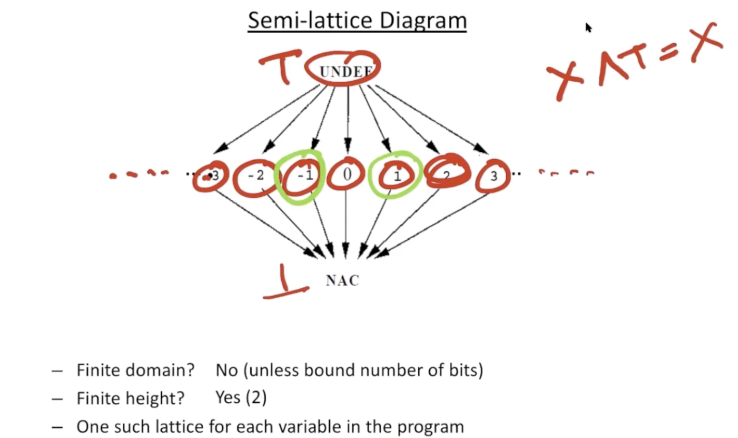
\includegraphics[width=0.3\textwidth]{p33.png}
    \caption{}
    \label{fig:p33}
\end{figure}

\subsubsection{Meet Operator in Table Form}
\begin{figure}[h]
    \centering
    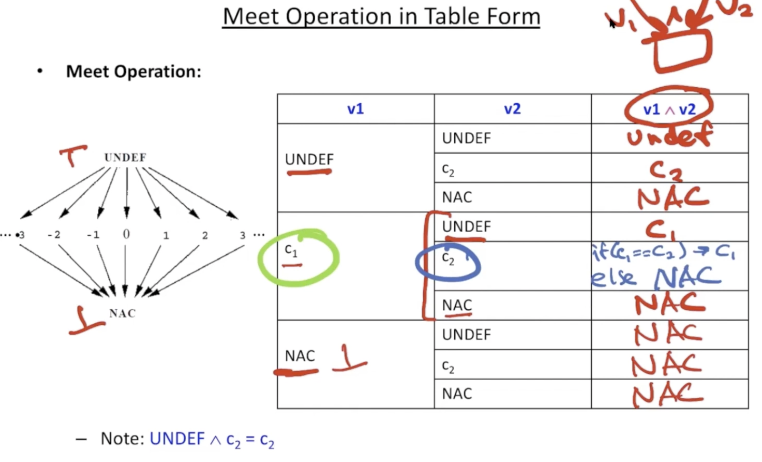
\includegraphics[width=0.3\textwidth]{p34.png}
    \caption{}
    \label{fig:p34}
\end{figure}


\subsubsection{Example}

\begin{figure}[h]
    \centering
    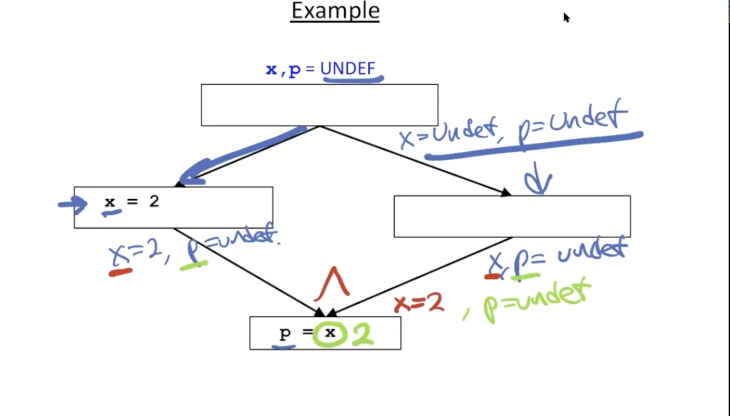
\includegraphics[width=0.3\textwidth]{p35.png}
    \caption{}
    \label{fig:p35}
\end{figure}

On the other path in \ref{fig:p35}, x is uninitialized. When we have undefined behavior, hopefully the front end of the compiler should complain about it, but if it doesn't, the optimizer is free to do whatever it wants to do.


\subsubsection{Transfer Function}


\begin{figure}[h]
    \centering
    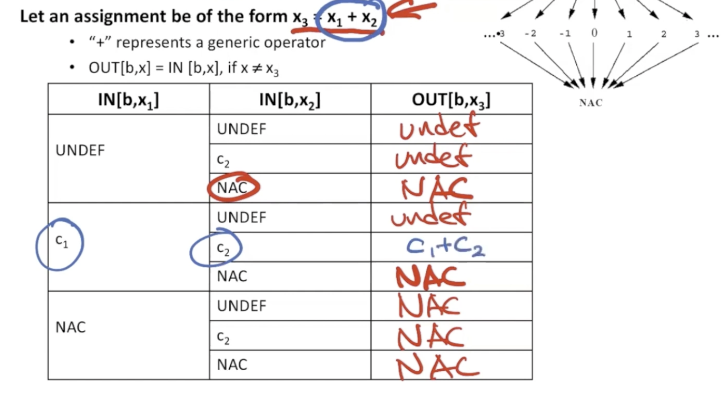
\includegraphics[width=0.3\textwidth]{p36.png}
    \caption{}
    \label{fig:p36}
\end{figure}



It is not distributive in \ref{fig:p37}.

\begin{figure}[h]
    \centering
    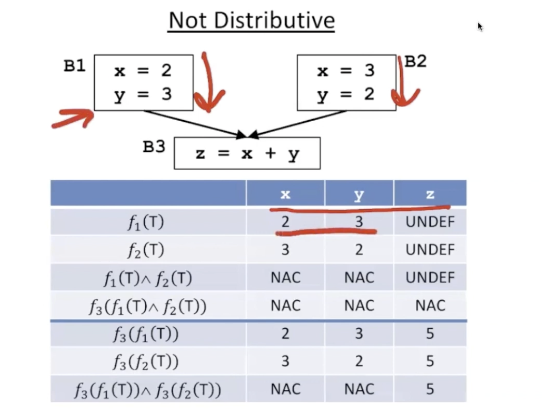
\includegraphics[width=0.3\textwidth]{p37.png}
    \caption{}
    \label{fig:p37}
\end{figure}



\subsection{Copy Propagation}

\subsection{Dead Code Elimination}




\section{Local Optimizations}

Local Optimizations never goes away because this is always a piece of what happens even when we 
talk about even more sophiscated types of optimizations.

First we will talk about how to represent the code within a function or procedure, that's using 
something called a flow graph which is made of basic blocks.  Next we will contrast two different 
abstractions for doing local optimizations.




\subsection{Basic Blocks/Flow graphs} 


\subsubsection{Basic Blocks}

A basic block is a sequence of instructions(3-address statements). There are some requirements for basic 
block:

\begin{itemize}
    \item \textbf{Only the first instruction can be reached from outside the blcok.} The reason why this property 
    is useful is that within a basic block, we just march instruction by instruction through the block, 
    this simplies things at least within a basic block.
    \item \textbf{All the statements are executed consecutively if the first one is.}
    \item \textbf{The basic block must be maximal.} i.e., they cannot be made larger without violating conditions. 
\end{itemize}


\subsubsection{Flow graphs}
Flow graph is a graph representation of the procedure. In flow graph, basic blocks are the nodes, and the edge for \(  B_i 
\rightarrow B_j \) stands for a path from node \( B_i \) to node \( B_j \). So how will \(  B_i  \rightarrow B_j \) happen? 
There are two possibilities:

\begin{itemize}
    \item Either first instruction of \(B_j\) is the target of a goto at end of \(B_i\).
    \item \(B_j\) physically follows \(B_i\) which doesn't end in an unconditional goto.
\end{itemize}




% \begin{center}

% \begin{tikzpicture}[auto,
%     node distance = 12mm,
%     start chain = going below,
%     box/.style = {draw,rounded corners,blur shadow,fill=white,
%           on chain,align=center}]
%    \node[box] (b1)    {$x_1\leftarrow0$\\ $y_1\leftarrow0$};      
%    \node[box] (b2)    {$x_2\leftarrow\phi(x_1,x_3)$\\
%    $y_2\leftarrow\phi(y_1,y_3)$\\
%    $(x_2<10)$?};      
%    \node[box] (b3)    {$y_3\leftarrow y_2+x_2$\\ $x_3\leftarrow x_2+1$};  
%    \node[box] (b4)    {print($y_2$)};     
%    \begin{scope}[rounded corners,-latex]
%     \path (b2.-40) edge[bend left=50] (b4.40)
%     (b1) edge (b2) (b2) edge (b3);
%     \draw (b3.230) -- ++(0,-0.3) -| ([xshift=-5mm]b2.west) |-
%     ([yshift=3mm]b2.130) -- (b2.130);
%    \end{scope}
%   \end{tikzpicture}

% \end{center}




\subsubsection{Partitioning into Basic Blocks}

\begin{itemize}
\item Identify the leader of each basic block 
    \begin{itemize}
        \item First instruction
        \item Any target of a jump
        \item Any instruction immediately following a jump
    \end{itemize}

\item Basic block starts at leader and ends at instruction immediately before a leader(or the last instruction).    
\end{itemize}

An example of flow graph is shown below:

\begin{figure}[h]
    \centering
    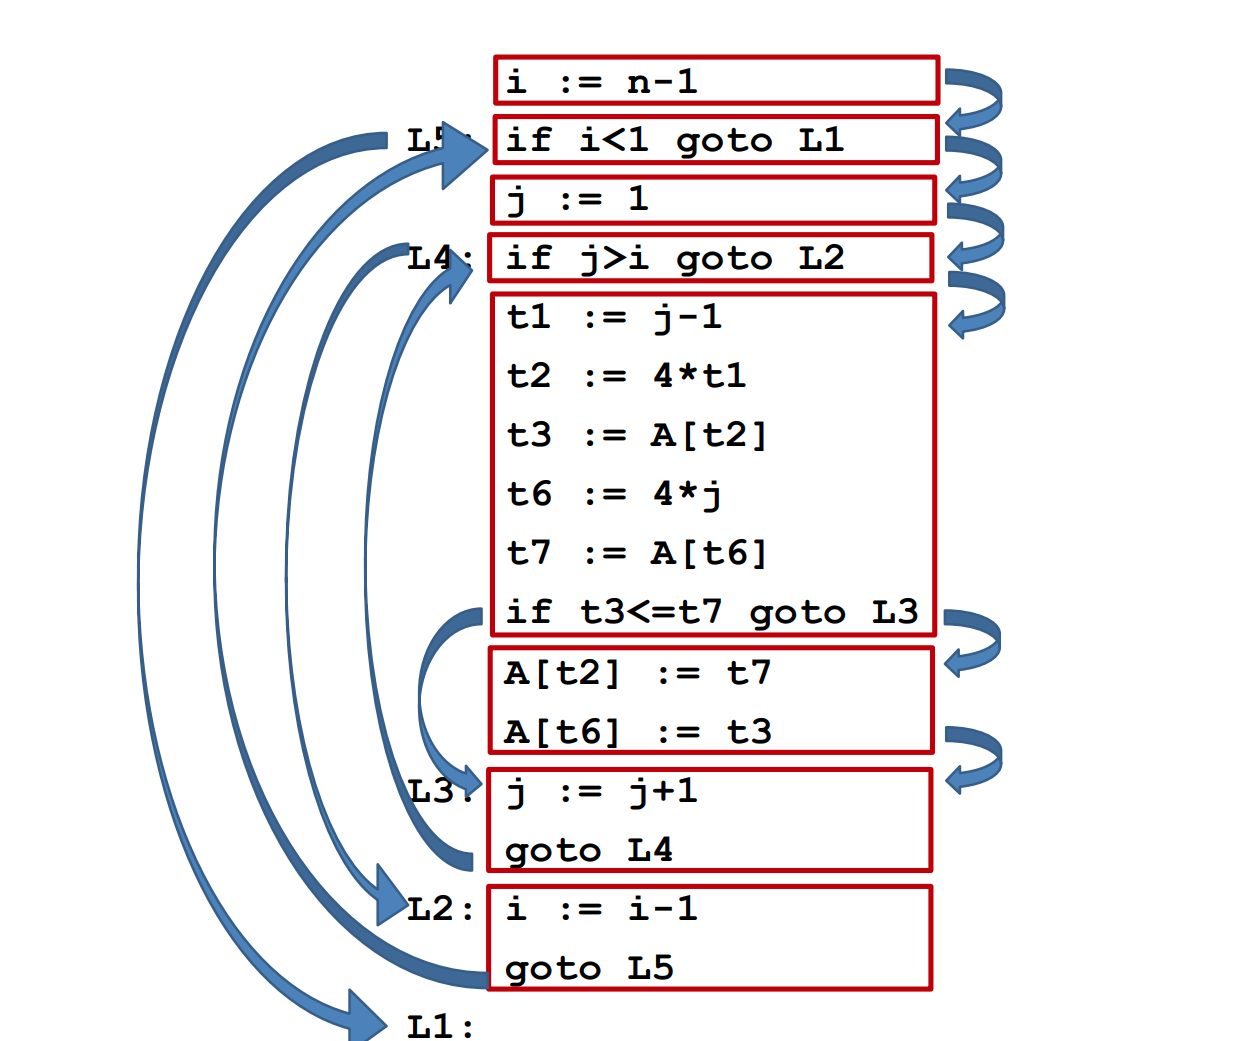
\includegraphics[width=0.5\textwidth]{flowgraph.png}
    \caption{Example of a flow graph}
\end{figure}

\subsubsection{Reachability of Basic Blocks}

There is one thing interesting need to mention here. So the source code is below:

\begin{lstlisting}[language=C, caption=An example]
if x { 
    ...
    return;
} else {
    ...
}


\end{lstlisting}


The corresponding flow graph is shown in \ref{fig:fgex}:

\begin{figure}[h]
    \centering
    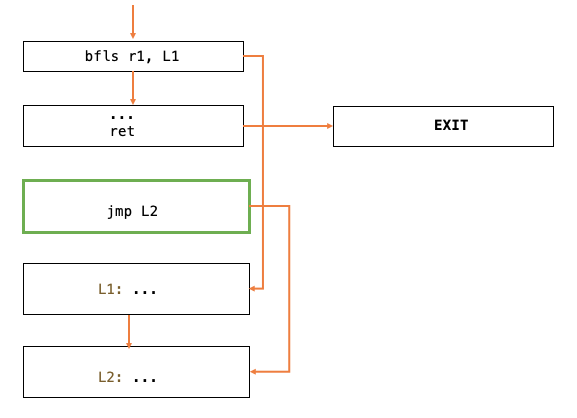
\includegraphics[width=0.5\textwidth]{fgex.png}
    \caption{Example of a flow graph}
    \label{fig:fgex}
\end{figure}


We can see that the box in green is unreachable from the entry. So why is that interesting? Typically, after compiers 
construct the control flow graph, they will go through and remove any unreachable nodes. Just do depth first traversal of the graph
from the entry node and mark all those visited nodes. So unmarked nodes will be deleted. This will help the compiler get a better optimization
result.


So why do these unreachable nodes appear? The anwser is it is not the job of the front-end of the compiler to clean up the unreachable nodes. 



\subsection{Local optimizations}

Local optimizations are those occur \textbf{within the basic blocks}. 


\subsubsection{common subexpression elimination}

There're some types of local optimizations. 
One is called \textbf{common subexpression elimination}. Subexpressions are some arithmetic expressions that occur on the
 right hand of the instructions. Common subexpressions are subexpression that occur many times where the operands have not 
 changed.
 
\begin{lstlisting}[language=C, caption=Subexpression example,label=lst:subexp]
a = b + c;
d = b + c;
\end{lstlisting}

In the example \ref{lst:subexp}, \texttt{b + c} is so called coomon subexpression, we could replace the instruction containing 
common subexpression with an assign expression. 


\begin{lstlisting}[language=C, caption=code snippet applied common subexpression elimination to \ref{lst:subexp},label=lst:transsubexpr]
    a = b + c;
    d = a
\end{lstlisting}

You may wonder why this kind of redundancy can occure in code? Are we programmers stupid to do so? In fact, 
the redundancy most comes from the stage when compilers  turn your source code. For example, when you use arrays,
you need to do some arithmetic to generate the address of the array element you are accessing. So every time you referece the same
array element, compiler will calculate the same address again. Similarly, if you access offsets within fields. Last example is 
access to parameters in the stack. 


\subsection{Abtraction 1:DAG}

DAG is the acronym for Directed Acyclic Graph. The Directed Acyclic Graph (DAG) is used to represent the 
structure of basic blocks, to visualize the flow of values between basic blocks, and to provide 
optimization techniques in the basic block. DAG is an efficient method for identifying common 
sub-expressions.\footnote{copied from \url{https://wildpartyofficial.com/what-is-dag-in-compiler-construction}}



The parse tree and DAG of the expression \(a + a*(b+c) + (b+c) *d \) is shown in \ref{fig:DAG}.


\begin{figure}[h]
    \centering
    \includegraphics[width=0.5\textwidth]{DAG.png}
    \caption{Example of a DAG}
    \label{fig:DAG}
\end{figure}



In DAG, some of the computation are reused. So we can generate optimizaed code based on DAG.

The optmized code for the DAG\ref{fig:DAG} is: 

\begin{lstlisting}[language=C, caption=code ,label=lst:dag]
    t1 = b - c;
    t2 = a * t1;
    t3 = a + t2;
    t4 = t1 * d;
    t5 = t3 + t4;
\end{lstlisting}


\subsubsection{How well do DAGs hold up across statements?}

We have seen that DAGs can be useful in a long arithmetic expression. So how well do DAGs
perform in sequence of instructions?

\begin{lstlisting}[language=C, caption=code ,label=lst:dagexpr2]
    a = b + c;
    b = a - d;
    c = b + c;
    d = a - d;
\end{lstlisting}


The corresponding DAG is shown in \ref{fig:DAG2}.
\begin{figure}[h]
    \centering
    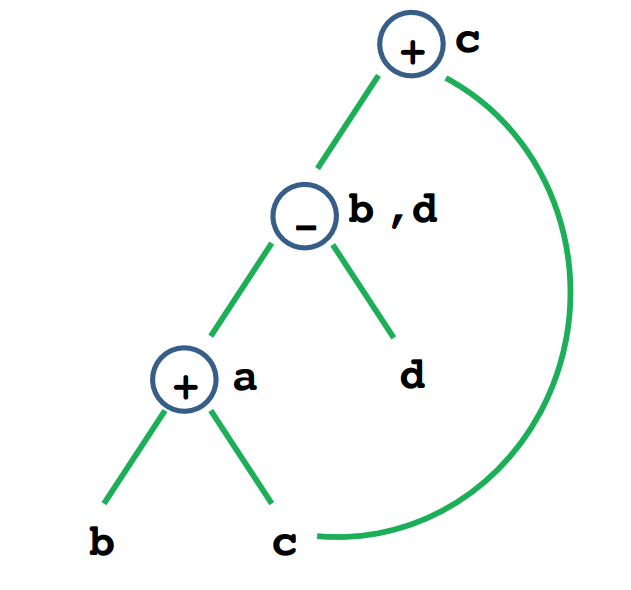
\includegraphics[width=0.5\textwidth]{dag2.png}
    \caption{Example of a DAG}
    \label{fig:DAG2}
\end{figure}

Based on the DAG\ref{fig:DAG2}, one optimizaed code is \ref{lst:dagexprop2}


\begin{lstlisting}[language=C, caption=code ,label=lst:dagexprop2]
a = b+c;
d = a-d;
c = d+c;
\end{lstlisting}

\ref{lst:dagexprop2} is not correct. B need to be overwritten but not yet. So if using DAGs, you need to be 
very careful. 

DAGs make sense if you just have one long expression, but once you have sequence of instructions overwriting variables
, DAGs are less appealing because this abstraction doesn't really include the concept of time.




\subsection{Abtraction 2:Value numbering} 

We have seen drawbacks of DAGs. One way to fix the problem is to attach variable name to latest value. Value numbering is 
such abstraction.

The idea behind value numbering is there is a mapping between variables(static) to values(dynamic). So common subexpression means same 
value number.

\subsubsection{Algorithm}


\begin{lstlisting}[language=python, caption=code ,label=lst:vna]
Data structure:
    VALUES = Table of
        expression /* [OP, valnum1, valnum2] */
        var /* name of variable currently holding expr */
For each instruction (dst = src1 OP src2) in execution order
    valnum1=var2value(src1); valnum2=var2value(src2)

    IF [OP, valnum1, valnum2] is in VALUES
        v = the index of expression
        Replace instruction with: dst = VALUES[v].var
    ELSE
        Add
            expression = [OP, valnum1, valnum2]
            var = tv
        to VALUES
        v = index of new entry; tv is new temporary for v
        Replace instruction with: tv = VALUES[valnum1].var OP VALUES[valnum2].var
                                dst = tv
    set_var2value (dst, v)  
\end{lstlisting}


\subsubsection{example}







\section{Introduction to Data Flow Analysis}

\subsection{Motivation for Dataflow Analysis}

Some optimizations\footnote{based on \url{https://pages.cs.wisc.edu/~horwitz/CS704-NOTES/2.DATAFLOW.html}} , however, require more "global" information. 
For example, consider the code \ref{lst:expr1}

\begin{lstlisting}[language=C,frame=single, caption=An ,label = lst:expr1]
    a = 1;
    b = 2;
    c = 3;
    if (...) x = a + 5;
    else x = b + 4;
    c = x + 1;
\end{lstlisting}


In this example, the initial assignment to \textit{c} (at line 3) is useless, and the expression 
\textit{x + 1} can be simplified to 7, but it is less obvious how a compiler can discover these facts 
since they cannot be discovered by looking only at one or two consecutive statements. 
A more global analysis is needed so that the compiler knows at each point in the program:
\begin{itemize}
\item    which variables are guaranteed to have constant values, and
\item    which variables will be used before being redefined.
\end{itemize}

To discover these kinds of properties, we use dataflow analysis. 



\subsubsection{What is Data Flow Analysis?}

Local Optimizations only consider optimizations within a node in CFG. 
Data flow analysis will take edges into account, which means composing 
effects of basic blocks to derive information at basic block boundaries.
Data-flow analysis is a technique for gathering information about the possible 
set of values calculated at various points in a computer program. A program's 
control-flow graph (CFG) is used to determine those parts of a program to which 
a particular value assigned to a variable might propagate. The information gathered 
is often used by compilers when optimizing a program. 


Typically, we will do local optimization for the first step to know what happens in a 
basic block, step 2 is to do data flow analysis. In he third step, we will go back and 
revisit the individual instructions inside of the blocks.


Data flow analysis is \textbf{flow-sensitive}, which means we take into account
 the effect of control flow. It is also a \textbf{intraprocedural analysis} which means
 the analysis is within a procedure. Data-flow analysis computes its solutions over the paths in
 a control-flow graph. The well-known, meet-over-all-paths
 formulation produces safe, precise solutions for general dataflow problems. All paths-whether feasible or infeasible,
 heavily or rarely executed-contribute equally to a solution. 

Here are some examples of intraprocedural optimizations:

\begin{itemize}
\item \textbf{constant propagation}. Constant propagation is a well-known global flow analysis 
problem. The goal of constant propagation is to discover values that are constant on all possible 
executions of a program and to propagate these constant values as far forward through the program 
as possible. Expressions whose operands are all constants can be evaluated at compile time and the 
results propagated further.

\item \textbf{common subexpression elimination}

\item \textbf{dead code elimination}. Actually, source code written by programmers doesn't contain
 a lot of dead code, dead code happens to occur partly because of how the front end translates code into 
 the IR. Doing optimizations will also turn code into dead.

\end{itemize}

% \subsection{Static    Program    vs.    Dynamic    Execution }

% Static program 




\subsubsection{Static Program vs. Dynamic Execution}


Program is statically infinite, but there can be infinite many dynamic execution paths. On one hand, analysis
 need to be precise, so we will take into account as much dynamic execution as possible. On the other hand, analysis
 need to do the analysis quickly. For a compromise, the analysis result is \textbf{conservative} and what it does id for each 
 point in the program, combines information of all the instances of the same program point.





\subsubsection{Data Flow Analysis Schema}
Before thinking about how to define a dataflow problem, note that there are two kinds of problems:
\begin{itemize}
    \item Forward problems (like constant propagation) where the information at a node n summarizes what can happen on paths from "enter" to n. So if we care about what happened in the past, it's a forward problem.
    \item Backward problems (like live-variable analysis), where the information at a node n summarizes what can happen on paths from n to "exit". So if we care about what will happen in the future, it's a backward problem.
\end{itemize}    

In what follows, we will assume that we're thinking about a forward problem unless otherwise specified.
 
Another way that many common dataflow problems can be categorized is as may problems or must problems. 
The solution to a "may" problem provides information about what may be true at each program point (e.g., 
for live-variables analysis, a variable is considered live after node n if its value may be used before 
being overwritten, while for constant propagation, the pair (x, v) holds before node n if x must have the value v at that point).

Now let's think about how to define a dataflow problem so that it's clear what the (best) solution should be. 
When we do dataflow analysis "by hand", we look at the CFG and think about:

\begin{itemize}
    \item What information holds at the start of the program.
    \item When a node n has more than one incoming edge in the CFG, how to combine the incoming 
    information (i.e., given the information that holds after each predecessor of n, how to 
    combine that information to determine what holds before n).
    \item How the execution of each node changes the information.
\end{itemize}    

This intuition leads to the following definition. An instance of a dataflow problem includes:
\begin{itemize}
    \item a \(CFG\),
    \item a domain \(D\) of "dataflow facts",
    \item a dataflow fact "init" (the information true at the start of the program for forward problems, 
    or at the end of the program for backward problems),
    \item an operator \(\wedge\) (used to combine incoming information from multiple predecessors),
    \item for each CFG node n, a dataflow function \(f_n\) :\( D \rightarrow D\) (that defines the effect of 
    executing n).
\end{itemize} 

For constant propagation, an individual dataflow fact is a set of pairs of the form (var, val),
 so the domain of dataflow facts is the set of all such sets of pairs (the power set). 
 For live-variable analysis, it is the power set of the set of variables in the program.

For both constant propagation and live-variable analysis, the "init" fact is the empty set 
(no variable starts with a constant value, and no variables are live at the end of the program).



For constant propagation, the combining operation \(\wedge\) is set intersection. 
This is because if a node n has two predecessors, p1 and p2, then variable x has value v before 
node n iff it has value v after both p1 and p2. For live-variable analysis, 
\(\wedge\) is set union: if a node n has two successors, s1 and s2, then the value of x after n may be 
used before being overwritten iff that holds either before s1 or before s2. In general, 
for "may" dataflow problems, \(\wedge\) will be some union-like operator, while it will be an intersection-like 
operator for "must" problems.

For constant propagation, the dataflow function associated with a CFG node that does not assign 
to any variable (e.g., a predicate) is the identity function. For a node n that assigns to 
a variable x, there are two possibilities:

\begin{itemize}
\item 1. The right-hand side has a variable that is not constant. In this case, the function 
result is the same as its input except that if variable x was constant the before n, 
it is not constant after n.
\item 2. All right-hand-side variables have constant values. In this case, the right-hand side of 
the assignment is evaluated producing consant-value c, and the dataflow-function result is the 
same as its input except that it includes the pair (x, c) for variable x (and excludes the pair 
for x, if any, that was in the input).
\end{itemize}


For live-variable analysis, the dataflow function for each node n has the form: 
\(f_n(S) = Gen_n \cup (S - KILL_n)\), where \(KILL_n\) is the set of variables defined at node n, 
and \(GEN_n\) is the set of variables used at node n. In other words, for a node that does not 
assign to any variable, the variables that are live before n are those that are live after 
n plus those that are used at n; for a node that assigns to variable x, the variables that are 
live before n are those that are live after n except x, plus those that are used at n 
(including x if it is used at n as well as being defined there).

An equivalent way of formulating the dataflow functions for live-variable analysis is: 
\(f_n(S) = (S \cap NOT-KILL_n) \cup GEN_n\), where \(NOT-KILL_n\) is the set of variables not defined
 at node n. The advantage of this formulation is that it permits the dataflow facts to be 
 represented using bit vectors, and the dataflow functions to be implemented using simple 
 bit-vector operations (and or).

It turns out that a number of interesting dataflow problems have dataflow functions of this 
same form, where \(GEN_n\) and \(KILL_n\) are sets whose definition depends only on n, and the combining 
operator \(\wedge\) is either union or intersection. These problems are called GEN/KILL problems, 
or bit-vector problems.




\subsection{Reaching Definitions}

The Reaching Definitions Problem is a data-flow problem used to answer the
following questions: Which definitions of a variable \textit{X} reach a given use of \textit{X} in
an expression? Is \textit{X} used anywhere before it is defined? A definition\textit{d} reaches a point \textit{p} if there exists path 
from the point immediately following \textit{d} to \textit{p} such that \textit{d} is not killed(overwritten) along that path.



\subsubsection{Iterative   Algorithm}

Here is the iterative  algorithm.



\begin{algorithm}
    \caption{Reaching Defintions:Iterative Algorithm}\label{alg:reachingdefiterative}
    \hspace*{\algorithmicindent} \textbf{Input: control flow graph CFG = (N, E, Entry, Exit) } \\
   
    
    \begin{algorithmic}
   
    \State out[Entry] = $\emptyset$ \algorithmiccomment{Boundary condition}

    \For{\texttt{each basic block B other than Entry}}
        \State \texttt{out[B] = $\emptyset$} \algorithmiccomment{Initialization for iterative algorithm }
    \EndFor
    \While{Changes to any out[] occur}
        \For{\texttt{each basic block B other than Entry}}
        \State \texttt{$in[B] =  \cup (out[p])$, for all predecessors p of B}
        \State \texttt{$out[B] = f_B(in[B])$} \algorithmiccomment{$out[B]=gen[B]\cup (in[B]-kill[B]) $ }
        \EndFor

    \EndWhile
    \end{algorithmic}
\end{algorithm}




\subsubsection{ Worklist   Algorithm}

\begin{algorithm}
    \caption{Reaching Defintions:Worklist Algorithm}\label{alg:reachingdefiterative}
    \hspace*{\algorithmicindent} \textbf{Input: control flow graph CFG = (N, E, Entry, Exit) } \\
   
    
    \begin{algorithmic}
   
    \State out[Entry] = $\emptyset$ \algorithmiccomment{Boundary condition}
    \State \textcolor{blue}{ChangedNodes = N}   
    \For{\texttt{each basic block B other than Entry}}
        \State \texttt{out[B] = $\emptyset$} \algorithmiccomment{Initialization for iterative algorithm }
    \EndFor
    \While{ChangedNodes $\neq \emptyset$}
        \State \textcolor{blue}{Remove i from ChangedNodes}
        \State $in[B] =  \cup (out[p])$, for all predecessors p of B
        \State \textcolor{blue}{$oldout = out[i]$}
        \State $out[i] = f_i(in[i])$ \algorithmiccomment{$out[i]=gen[i]\cup (in[i]-kill[i]) $ }
        \If {\textcolor{blue}{oldout} $\neq out[i]$}

            \For{\texttt{all \textcolor{blue}{successors s of i}}}
                \State \textcolor{blue}{add s to ChangedNodes}
            \EndFor
        \EndIf

    \EndWhile
    \end{algorithmic}
\end{algorithm}



\subsubsection{Example}


\begin{figure}[!htb]
    \minipage{0.32\textwidth}
      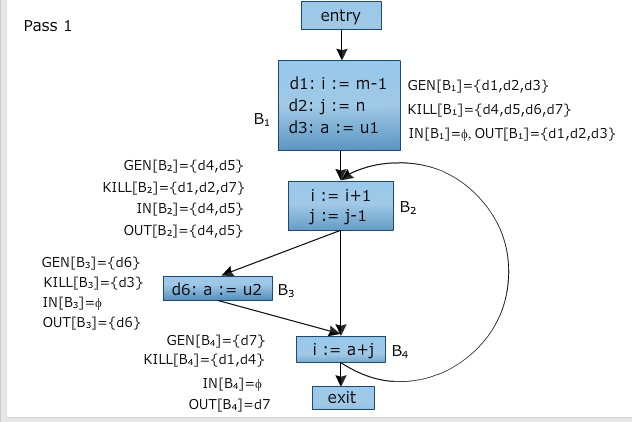
\includegraphics[width=\linewidth]{rdex1.jpg}
      \caption{Pass 1}\label{fig:awesome_image1}
    \endminipage\hfill
    \minipage{0.32\textwidth}
      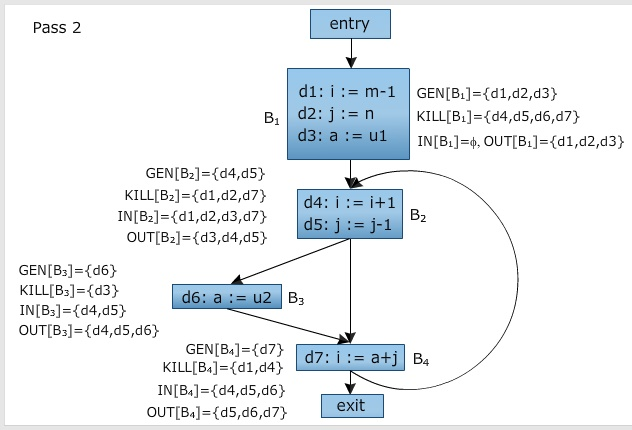
\includegraphics[width=\linewidth]{rdex2.jpg}
      \caption{Pass 2}\label{fig:awesome_image2}
    \endminipage\hfill
    \minipage{0.32\textwidth}%
      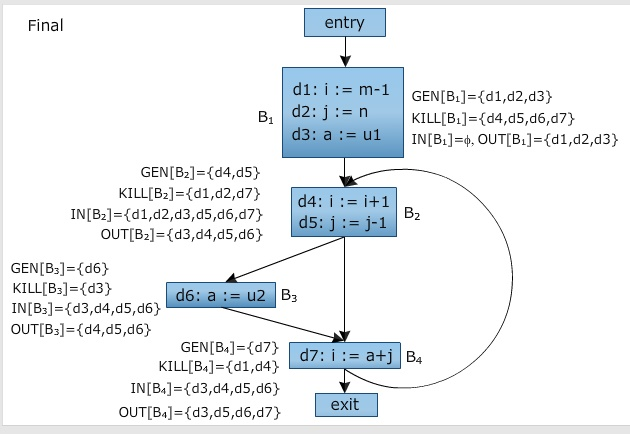
\includegraphics[width=\linewidth]{rdex3.jpg}
      \caption{Pass 3}\label{fig:awesome_image3}
    \endminipage
\end{figure}



\subsection{ Live    Variable    Analysis   }

In compilers, live variable analysis (or simply liveness analysis)
 is a classic data-flow analysis to calculate the variables that 
 are live at each point in the program. A variable is live at 
 some point if it holds a value that may be needed in the future, 
 or equivalently if its value may be read before the next time 
 the variable is written to. \footnote{based on Wikipedia}

\subsubsection{Motivation}


For dead code elimination.
\subsection{}


\section{ Live Variabl Analysis   }

In compilers, live variable analysis (or simply liveness analysis)
is a classic data-flow analysis to calculate the variables that
are live at each point in the program. A variable is live at
some point if it holds a value that may be needed in the future,
or equivalently if its value may be read before the next time
the variable is written to. \footnote{based on Wikipedia}

\subsection{Motivation}

Programs may contain

\begin{itemize}
	\item code which gets executed but which has no useful
	      effect on the program's overall result;
	\item occurrences of variables being used before they
	      are defined;\footnote{we can use liveness information to find undefined variables.}
	\item many variables which need to be allocated
	      registers and/or memory locations for compilation.\footnote{Two	variables	can	use	the	same	register	if	they	are	never	in	use	at	the
		      same time(i.e,	never	simultaneously live). Register	allocation
		      uses liveness information.}

\end{itemize}

The concept of variable liveness is useful in dealing
with all three of these situations.


Liveness analysis is highly used for \textbf{register allocation}(If variable \texttt{x} is live in a basic block b, it is a potential candidate for
register allocation) and \textbf{dead code elimination}(If variable \texttt{x} is not live after an assignment \texttt{x =...}, then the assignment is
redundant and can be deleted as dead code).


\subsection{Problem formulation}
Liveness is a data-flow property of variables:
“Is the value of this variable needed?” We therefore
usually consider liveness from an instruction's
perspective: each instruction (or node of the
flowgraph) has an associated set of live variables.


\subsection{Semantic vs. syntactic}


There are two kinds of variable liveness : Semantic liveness and Syntactic liveness.


A variable x is \textbf{semantically} live at a node n if there is
some execution sequence starting at n whose (externally
observable) behaviour can be affected by changing the
value of x. Semantic liveness is concerned with
the execution behaviour of the program.

A variable is \textbf{syntactically} live at a node if there is a
path to the exit of the flow graph along which its
value may be used before it is redefined. Syntactic liveness is concerned with properties of
the syntactic structure of the program.


So what is the difference between Semantic liveness and Syntactic liveness? syntactic liveness
is a computable approximation of semantic liveness.


Consider the example \ref{lst:expr2}


\begin{lstlisting}[language=C,frame=single, caption=An example to illustrate semantic syntatic,label = lst:expr2]
    int t = x * y;
    if ((x+1)*(x+1) == y) {
     t = 1;
    }
    if (x*x + 2*x + 1 != y) {
     t = 2;
    }
    return t;
\end{lstlisting}

In fact, t is dead in node \texttt{int t = x * y;} because one of the conditions will be true,
so on every execution path t is redefined before it is returned.
The value assigned by the first instruction is never used.


But on read path from Figure \ref{fig:liveex} through the
flowgraph, t is not
redefined before it's used,
so t is syntactically live at
the first instruction.Note that this path never
actually occurs during
execution.

\begin{figure}[h]
	\centering
	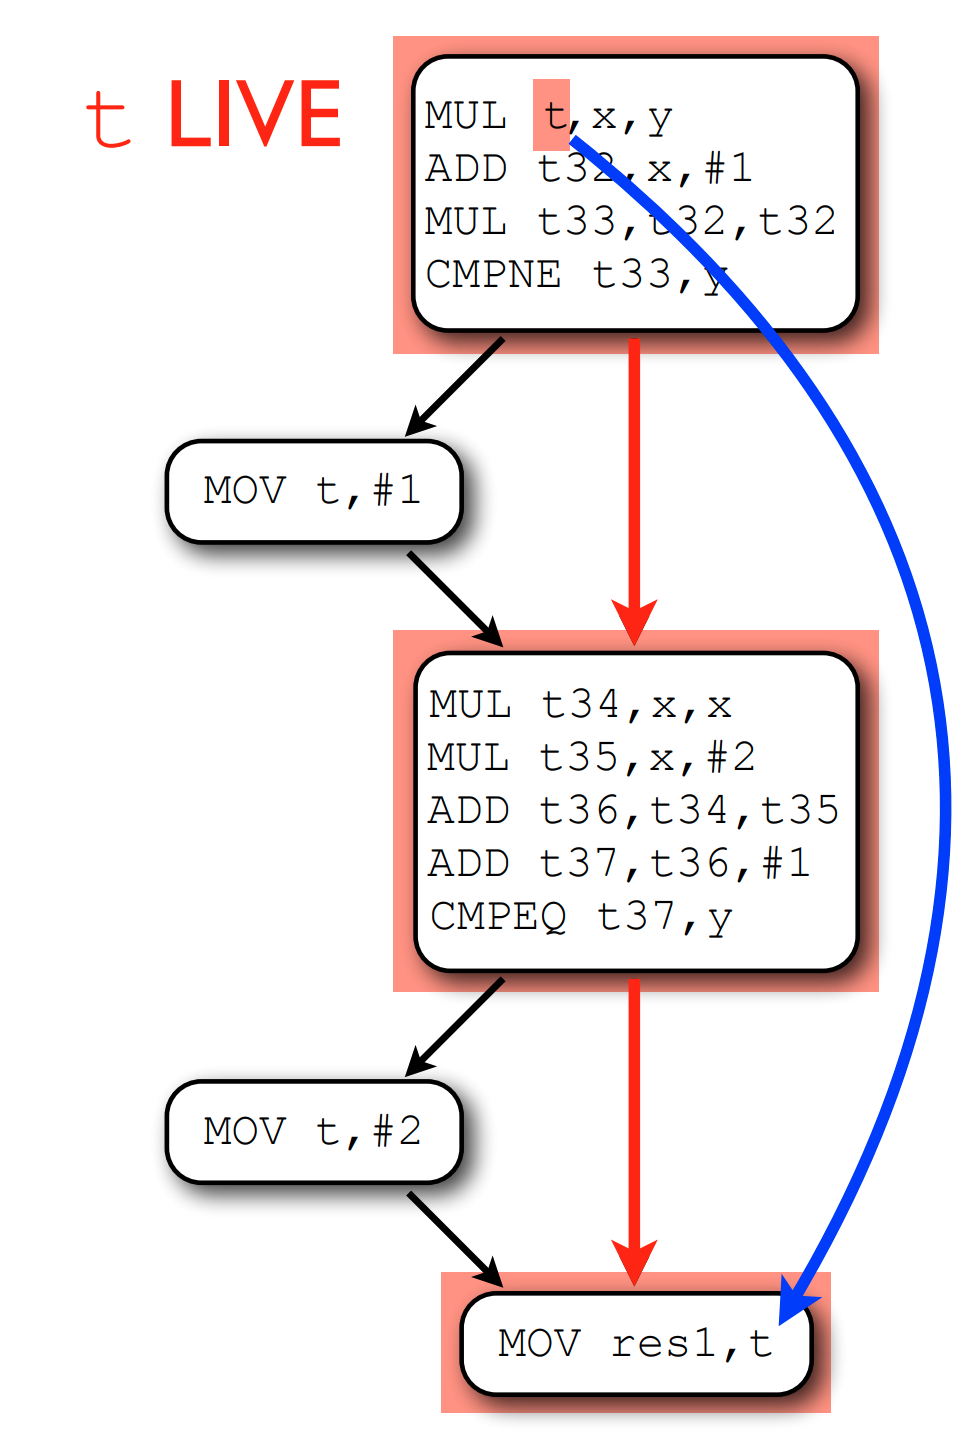
\includegraphics[width=0.3\textwidth]{liveex.png}
	\caption{CFG for \ref{lst:expr2}}
	\label{fig:liveex}
\end{figure}


\subsection{Summary}


\begin{center}
	\begin{tabular}{|c|c|}
		\hline Direction                         & Backward                                            \\
		\hline Domain                            & Sets	of	variables                                     \\
		\hline Meet operator                     & \( \cup \)                                          \\
		\hline Top(T)                            & $\phi$                                              \\
		\hline Bottom                            & Universal Set                                       \\
		\hline Boundary condition                & $\mathrm{IN[EXIT]} = \phi$                          \\
		\hline Initialization for internal nodes & $\mathrm{IN[B]} = \phi$                             \\
		\hline Finited escending chain?          & \checkmark                                          \\
		\hline Transfer function                 & $f_b(x) = \mathrm{USE}_b \cup (x - \mathrm{DEF}_b)$ \\
		\hline Monotone\&Distributive?           & \checkmark                                          \\
		\hline
	\end{tabular}
\end{center}




\subsection{Strongly Live Variables Analysis\cite{LiveVari29:online}}

A variable is strongly live if
\begin{itemize}

	\item it is used in a statement other than assignment statement, or
	      (same as simple liveness)
	\item it is used in an assignment statement defining a variable that is
	      strongly live
\end{itemize}


\begin{figure}[H]
	\centering
	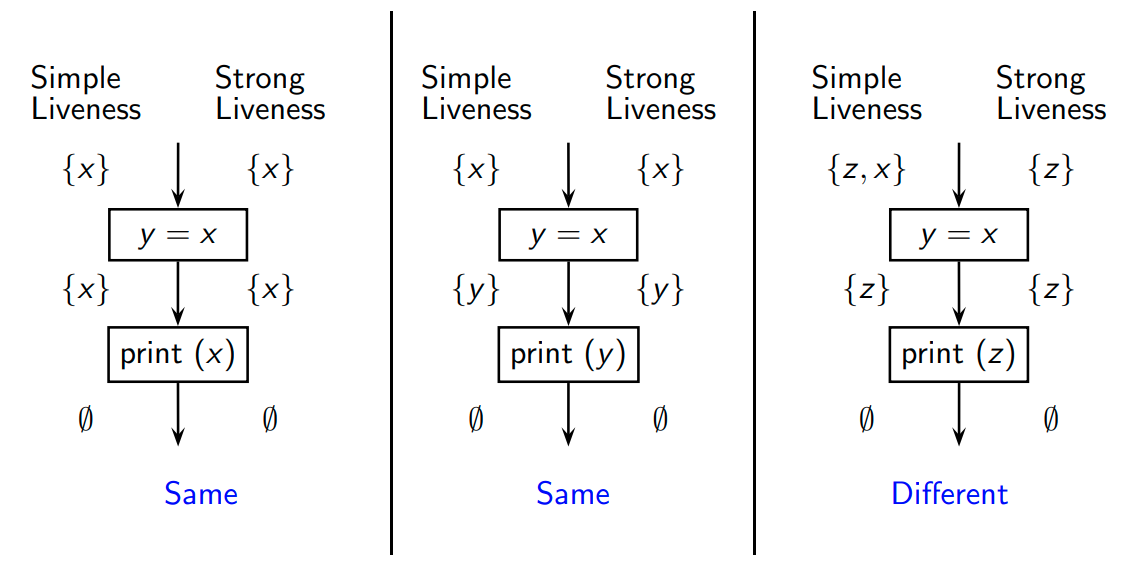
\includegraphics[width=0.7\textwidth]{p217.png}
	\caption{Understanding Strong Liveness}
	\label{fig:p217}
\end{figure}


A variable is live at a program
point if its current value is likely
to be used later. We want to compute the smallest
set of variables that are live. Simple liveness considers every
use of a variable as useful. Strong liveness checks the liveness
of the result before declaring the
operands to be live. Strong liveness is more precise
than simple liveness. The transfer function of Strongly Live Variables Analysis is shwon
below:


$$
	f_n(X)= \begin{cases}(X-\{y\}) \cup(Opd(e) \cap \mathbb{V}ar) & n \text { is } y=e, e \in \mathbb{E}pr, y \in X \\ X-\{y\} & n \text { is input }(y) \\ X \cup\{y\} & n \text { is use }(y) \\ X & \text { otherwise }\end{cases}
$$


The first case means that If \texttt{y} is not strongly live, the
assignment is skipped using
the “otherwise” clause

\begin{figure}[H]
	\centering
	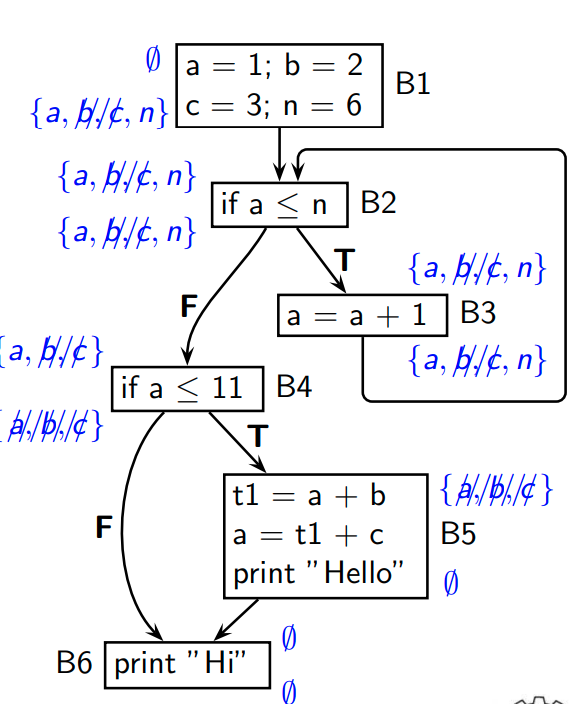
\includegraphics[width=0.4\textwidth]{p218.png}
	\caption{Simple Liveness VS. Strong Liveness.}
	\label{fig:p218}
\end{figure}

\section{Reaching Definitions}

The Reaching Definitions Problem is a data-flow problem used to answer the
following questions: Which definitions of a variable \textit{X} reach a given use of \textit{X} in
an expression? Is \textit{X} used anywhere before it is defined? A definition\textit{d} reaches a point \textit{p} if there exists path 
from the point immediately following \textit{d} to \textit{p} such that \textit{d} is not killed(overwritten) along that path.



\subsection{Iterative   Algorithm}

Here is the iterative  algorithm.



\begin{algorithm}
    \caption{Reaching Defintions:Iterative Algorithm}\label{alg:reachingdefiterative}
    \hspace*{\algorithmicindent} \textbf{Input: control flow graph CFG = (N, E, Entry, Exit) } \\
   
    
    \begin{algorithmic}
   
    \State out[Entry] = $\emptyset$ \algorithmiccomment{Boundary condition}

    \For{\texttt{each basic block B other than Entry}}
        \State \texttt{out[B] = $\emptyset$} \algorithmiccomment{Initialization for iterative algorithm }
    \EndFor
    \While{Changes to any out[] occur}
        \For{\texttt{each basic block B other than Entry}}
        \State \texttt{$in[B] =  \cup (out[p])$, for all predecessors p of B}
        \State \texttt{$out[B] = f_B(in[B])$} \algorithmiccomment{$out[B]=gen[B]\cup (in[B]-kill[B]) $ }
        \EndFor

    \EndWhile
    \end{algorithmic}
\end{algorithm}




\subsection{ Worklist   Algorithm}

\begin{algorithm}
    \caption{Reaching Defintions:Worklist Algorithm}\label{alg:reachingdefiterative}
    \hspace*{\algorithmicindent} \textbf{Input: control flow graph CFG = (N, E, Entry, Exit) } \\
   
    
    \begin{algorithmic}
   
    \State out[Entry] = $\emptyset$ \algorithmiccomment{Boundary condition}
    \State \textcolor{blue}{ChangedNodes = N}   
    \For{\texttt{each basic block B other than Entry}}
        \State \texttt{out[B] = $\emptyset$} \algorithmiccomment{Initialization for iterative algorithm }
    \EndFor
    \While{ChangedNodes $\neq \emptyset$}
        \State \textcolor{blue}{Remove i from ChangedNodes}
        \State $in[B] =  \cup (out[p])$, for all predecessors p of B
        \State \textcolor{blue}{$oldout = out[i]$}
        \State $out[i] = f_i(in[i])$ \algorithmiccomment{$out[i]=gen[i]\cup (in[i]-kill[i]) $ }
        \If {\textcolor{blue}{oldout} $\neq out[i]$}

            \For{\texttt{all \textcolor{blue}{successors s of i}}}
                \State \textcolor{blue}{add s to ChangedNodes}
            \EndFor
        \EndIf

    \EndWhile
    \end{algorithmic}
\end{algorithm}



\subsection{Example}
Here comes an example of reaching definition.

\begin{figure}[!htb]
    \minipage{0.32\textwidth}
      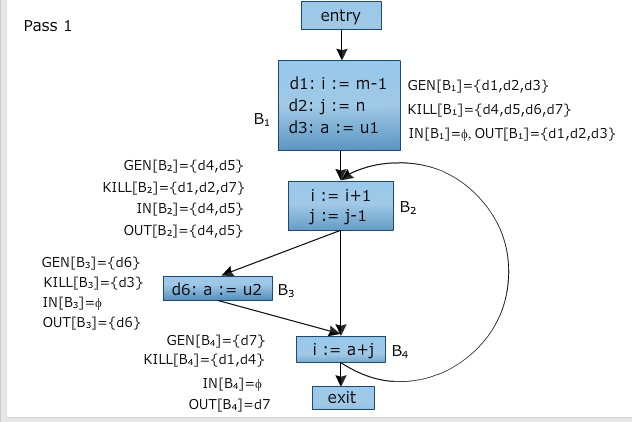
\includegraphics[width=\linewidth]{rdex1.jpg}
      \caption{Pass 1}\label{fig:awesome_image1}
    \endminipage\hfill
    \minipage{0.32\textwidth}
      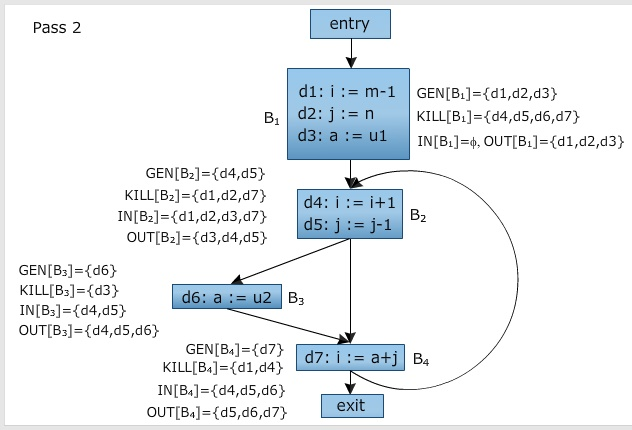
\includegraphics[width=\linewidth]{rdex2.jpg}
      \caption{Pass 2}\label{fig:awesome_image2}
    \endminipage\hfill
    \minipage{0.32\textwidth}%
      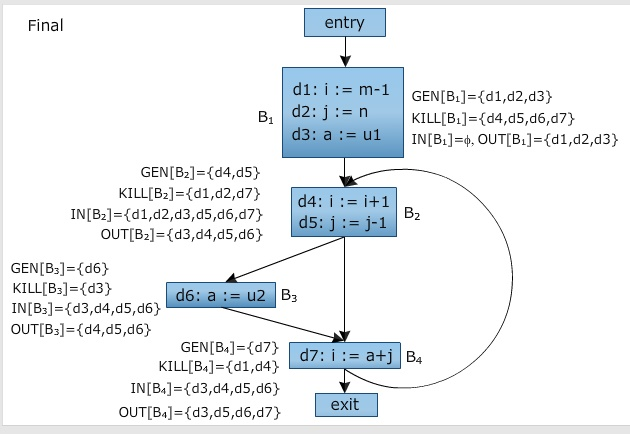
\includegraphics[width=\linewidth]{rdex3.jpg}
      \caption{Pass 3}\label{fig:awesome_image3}
    \endminipage
\end{figure}
\newpage

\section{Available Expressions Analysis}

\subsection{Motivation}

Programs may contain code whose result is needed, but in which some computation is simply a redundant
repetition of earlier computation within the same program. The concept of expression availability is useful in dealing with this situation.


\subsection{Backgroud Knowledge}

Any given program contains a finite number of expressions (i.e. computations which potentially
produce values),so we may talk about the set of all expressions of a program. Consider the program in
\ref{lst:expression1}




\begin{lstlisting}[language=C,frame=single, caption=An simple example containing some expressions ,label = lst:expression1]
    int z = x * y; 
    print s + t; 
    int w = u / v;
\end{lstlisting}


This program contian expression \texttt{x*y,s+t,u/v}.



\subsection{Problem Formulation}


Availability is a data-flow property of expressions: “Has the value of this expression already been computed?”
At each instruction, each expression in the programis either available or unavailable. So each instruction(or node of the flowgraph) has
an associated set of available expression.



\subsection{Semantic vs. Syntactic}

An expression is \textit{semantically} available at a node n if its value gets computed
(and not subsequently invalidated) along every execution sequence ending at n.

\begin{figure}[!htb]
	\minipage{0.5\textwidth}
	
\includegraphics[width=\linewidth]{p1.png}
	\caption{Available expression example}\label{fig:p1}
	\endminipage\hfill
	\minipage{0.5\textwidth}
	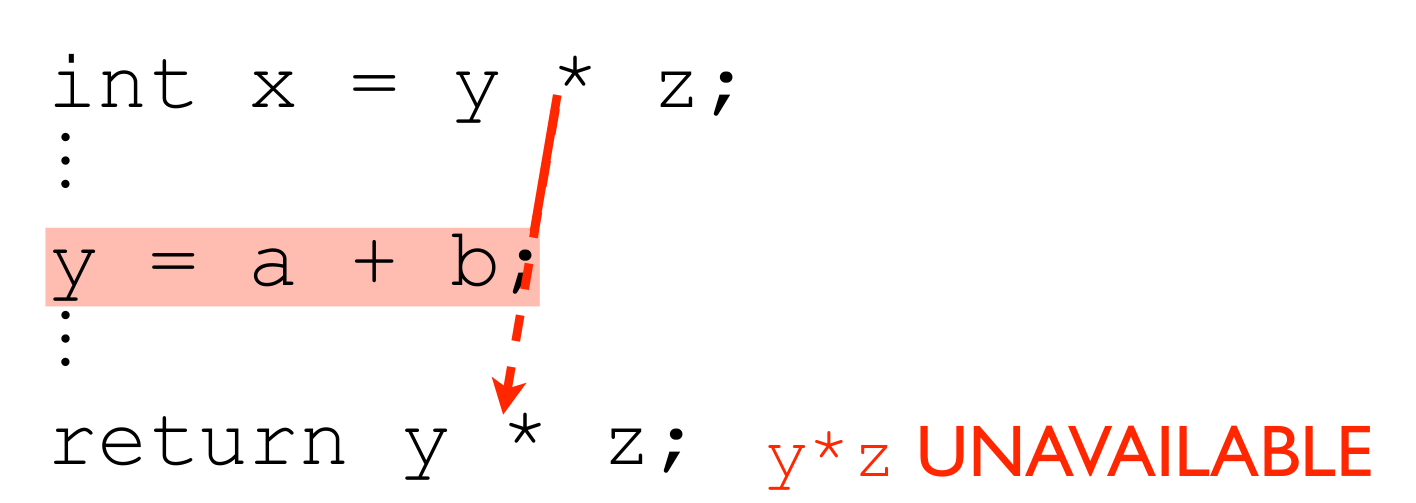
\includegraphics[width=\linewidth]{p2.png}
	\caption{unavailable expression example}\label{fig:p2}
	\endminipage
\end{figure}


An expression is \textit{syntactically} available at a node n if its value gets computed
(and not subsequently invalidated) along every path from the entry of the flowgraph to n.


\begin{figure}[!htb]
	\minipage{0.5\textwidth}
	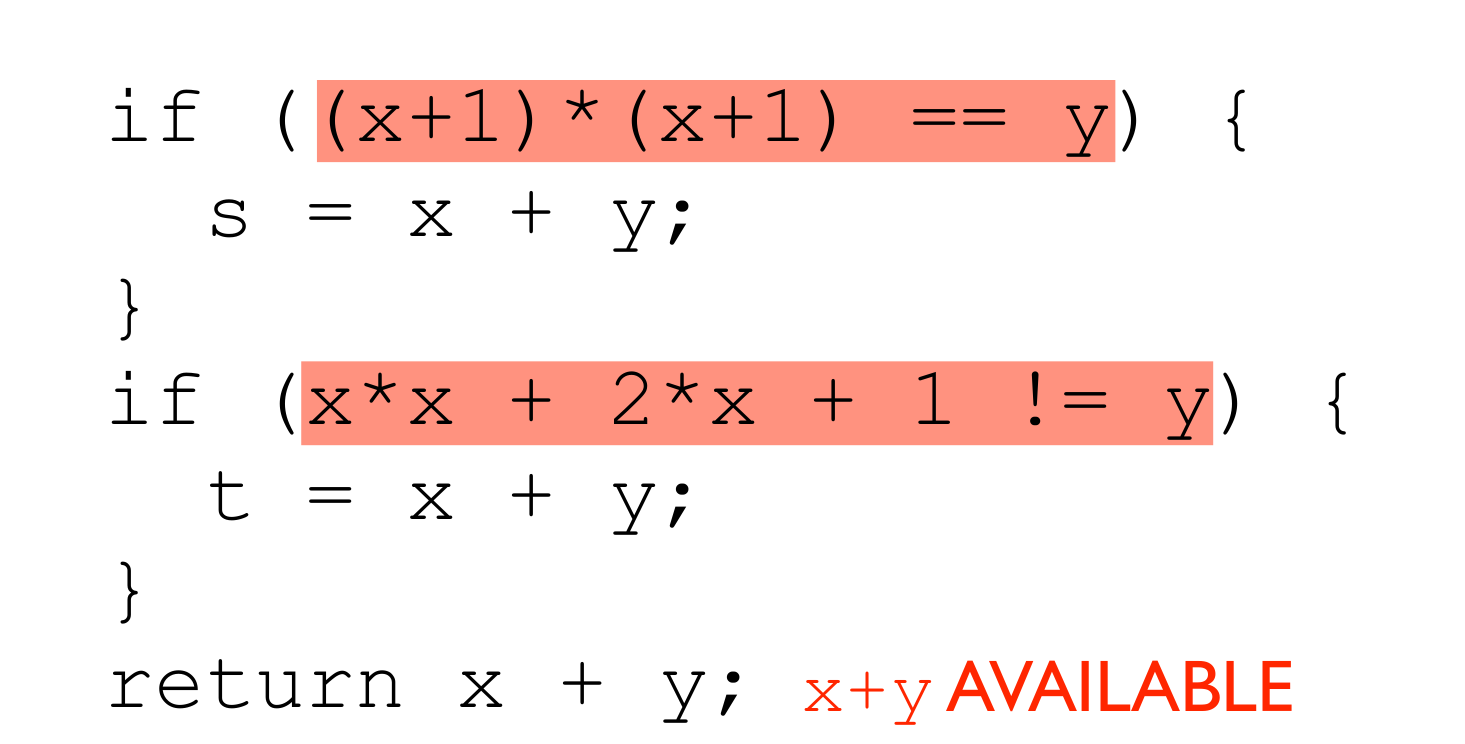
\includegraphics[width=\linewidth]{p4.png}
	\caption{x+y is semantically available}\label{fig:p4}
	\endminipage\hfill
	\minipage{0.4\textwidth}
	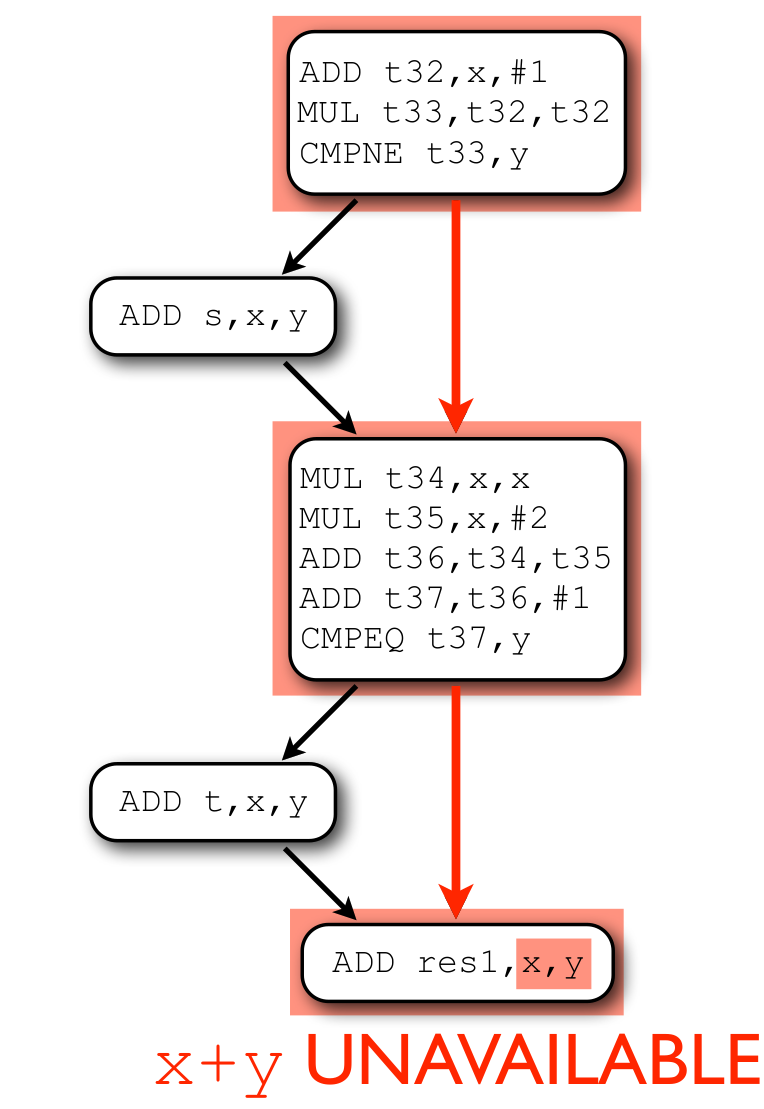
\includegraphics[width=\linewidth]{p3.png}
	\caption{x+y is syntactically unavailable}\label{fig:p3}
	\endminipage
\end{figure}


On the path in red from Figure \ref{fig:p3} through the flowgraph, \(x+y\) is only
computed once, so \(x+y\) is syntactically unavailable at the last instruction.


Whereas with live variable analysis we found safety in assuming that
more variables were live, here we find safety in assuming that fewer
expressions are available. Because if an expression is deemed to be available, we
may do something dangerous (e.g. remove an instruction which recomputes its value).
So sometimes safe means more, but sometimes means less.

\begin{figure}[H]
	\minipage{0.5\textwidth}
	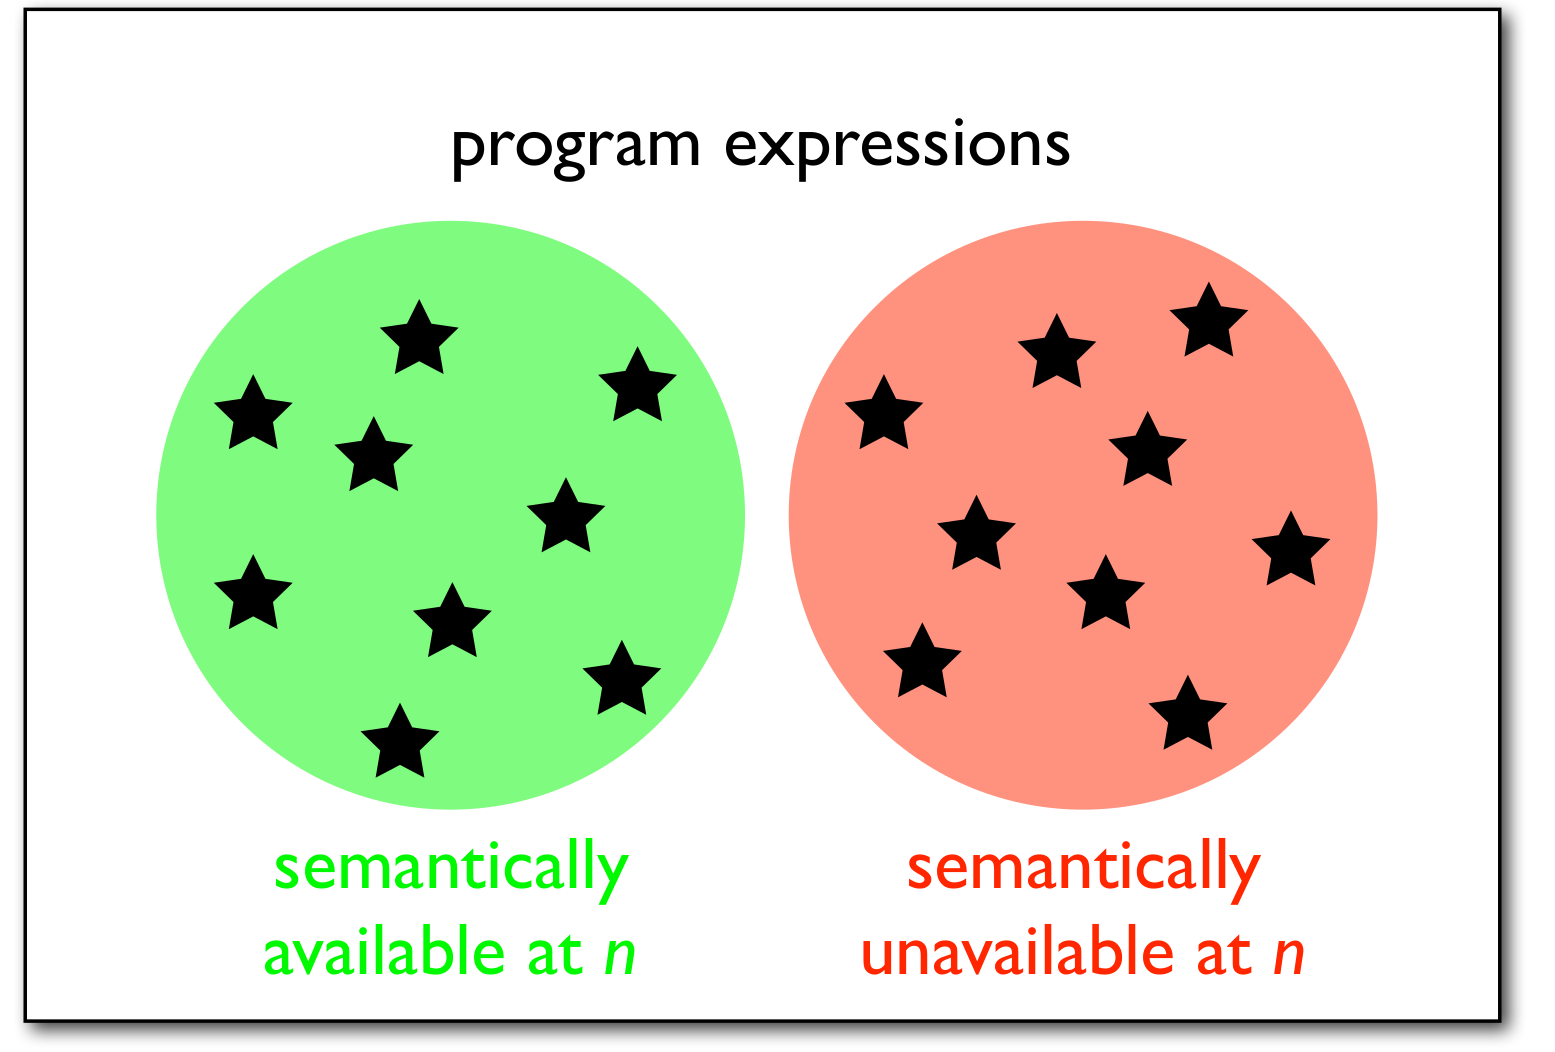
\includegraphics[width=\linewidth]{p5.png}
	\caption{Semantic vs. syntactic}\label{fig:p5}
	\endminipage\hfill
	\minipage{0.5\textwidth}
	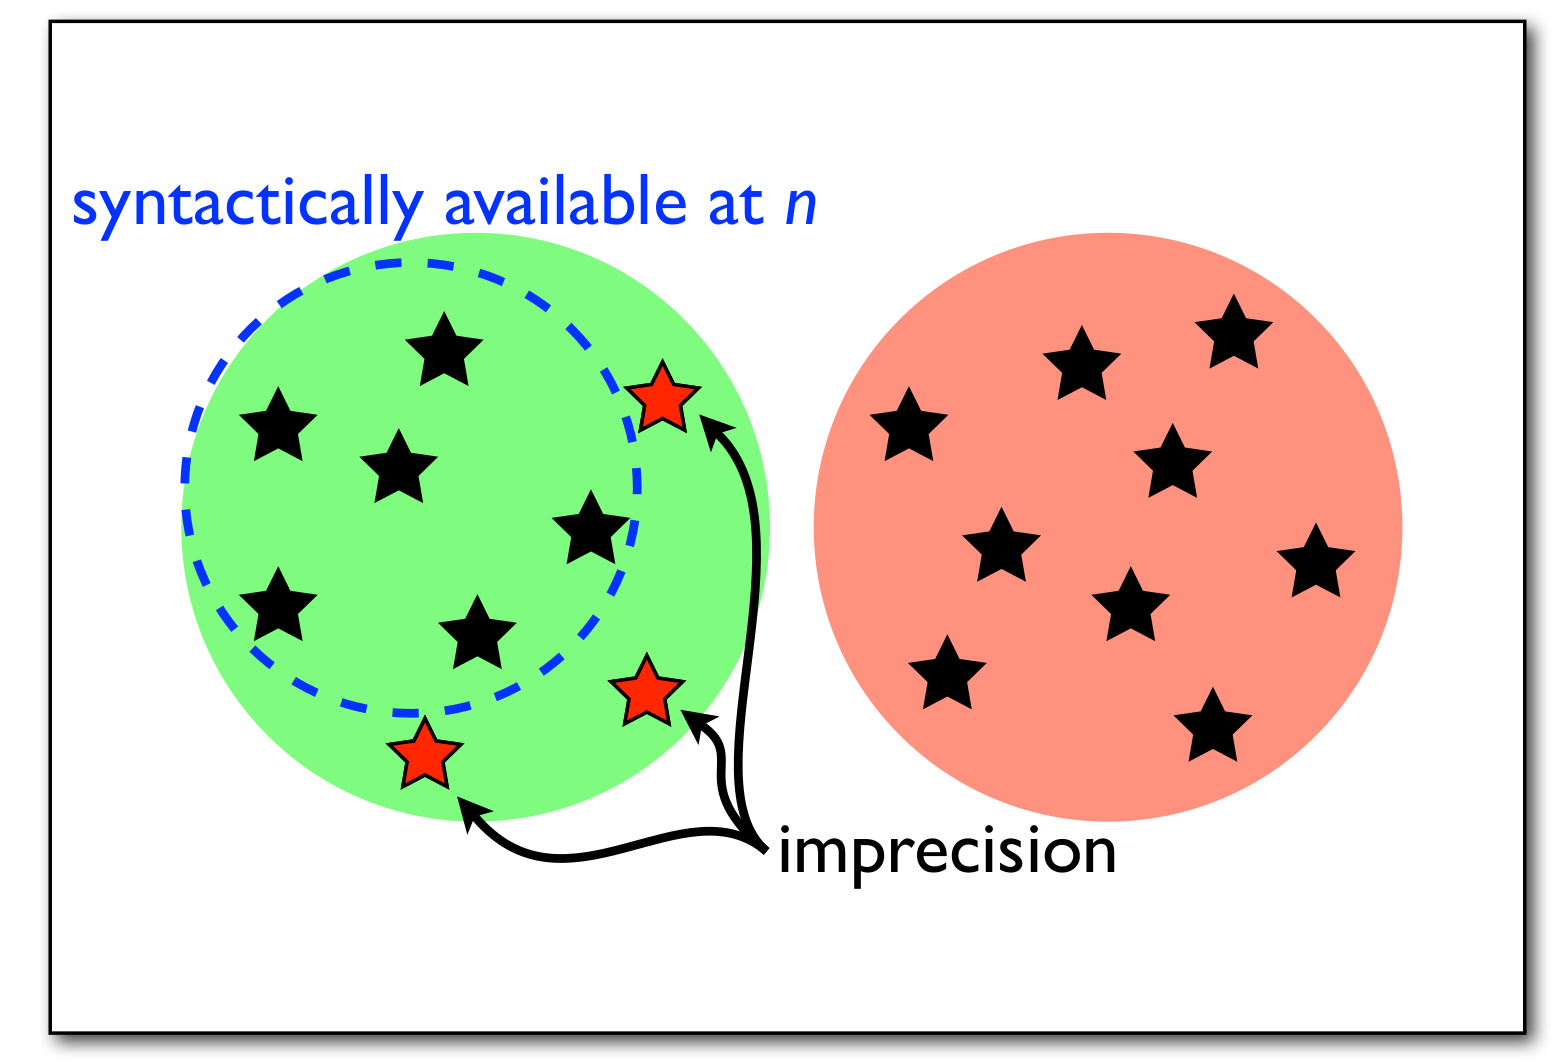
\includegraphics[width=\linewidth]{p6.png}
	\caption{Semantic vs. syntactic}\label{fig:p6}
	\endminipage
\end{figure}


\subsection{Summary}


\begin{center}
	\begin{tabular}{|c|c|}
		\hline Direction                         & Forward                                           \\
		\hline Domain                            & Sets of expressions                                    \\
		\hline Meet operator                     & \( \cap \)                                          \\
		\hline Top(T)                            & Universal Set                                             \\
		\hline Bottom                            & $\phi$                                     \\
		\hline Boundary condition                & $\mathrm{OUT[ENTRY]} = \phi$                          \\
		\hline Initialization for internal nodes & $\mathrm{OUT[B]} = T$                             \\
		\hline Finited escending chain?          & \checkmark                                          \\
		\hline Transfer function                 & $f_b(x) = \mathrm{Gen}_b \cup (x - \mathrm{Kill}_b)$ \\
		\hline Monotone\&Distributive?           & \checkmark                                          \\
		\hline $\mathrm{Kill}_b$ & all E such that block b defines a variable in E \\
    \hline $\mathrm{Gen}_b$ & all E such that block b evaluates E and doesn’t later kill it \\
    \hline
	\end{tabular}
\end{center}
\section{Foundations of Data Flow Analysis}



Having shown several useful examples of the data-flow abstraction, 
we now study the family of data-flow schemas as a whole, abstractly. 
We shall answer several basic questions about data-flow algorithms formally:

\begin{itemize}

\item Under what circumstances is the iterative algorithm used in data-flow analysis correct?
\item How precise is the solution obtained by the iterative algorithm?
\item Will the iterative algorithm converge?
\item How fast is the convergence?
\end{itemize}


\subsection{Partial Order}\footnote{Based on \url{https://pages.cs.wisc.edu/~horwitz/CS704-NOTES/2.DATAFLOW.html}}

A binary relation R on a set S is called a partial ordering(poset), or partial order if and only if it is:

\begin{itemize}
\item \textbf{Reflexive} \(x \leq x\)
\item \textbf{Antisymmetric} if \(x \leq y\) and \(y \leq x\) then \(x = y\)
\item \textbf{Transitive} if \(x \leq y\) and \(y \leq z\) then \(x \leq z\)
\end{itemize} 



\subsection{Lattices}

A lattice is a poset in which every pair of elements has:

\begin{itemize}
\item a Least Upper Bound (the join of the two elements), and
\item a Greatest Lower Bound (the meet of the two elements).
\end{itemize}    



\subsection{Complete lattices}


A complete lattice is a lattice in which all subsets have a greatest lower bound 
and a least upper bound (the bounds must be in the lattice, but not necessarily 
in the subsets themselves). Note that Every finite lattice (i.e., S is finite) is complete.


\subsection{Monotonic and distributive functions}

A function f: L → L (where L is a lattice) is monotonic iff for all x,y in L: x ⊆ y implies f(x) ⊆ f(y).

A function f: L → L (where L is a lattice) is distributive iff for all x,y in L: f(x meet y) = f(x) meet f(y).

Every distributive function is also monotonic (proving that could be good practice!) but not vice versa. For the GEN/KILL dataflow problems, all dataflow functions are distributive. For constant propagation, all functions are monotonic, but not all functions are distributive.


\subsection{Fixed points}

x is a fixed point of function f iff f(x) = x.

\subsection{Meet Operator}



\newpage

\newpage
\newpage
\newpage

\section{Introduction to Static Single Assignment}

Many dataflow analyses need to find the use-sites of each defined variable or the definition-sites of each variable used in an expression. The \textit{def-use chain} is a data structure that makes this efficient: for each statement in the flow graph, the compiler can keep a list of pointers to all the use sites of variables defined there, and a list of pointers to all definition sites of the variables used there. An improvement on the idea of def-use chains is static single-assignment form, or SSA form, an intermediate representation in which each variable has only one definition in the program text. SSA is very useful for many optimizations such as Loop-Invariant Code Motion and Copy Propagation.

% \subsection{Motivation}

% \begin{itemize}
%     \item The values in reused locations may be provably independent.
%     \item It would be nice if we could traverse directly between related uses and def's
% \end{itemize}

\subsection{Definition-Use and Use-Definition Chains}


\begin{definition}{Use-Definition (UD) Chains}
For a given definition of a variable X, what are all of its uses?

\end{definition}



\begin{definition}{Definition-Use (DU) Chains}
For a given use of a variable X, what are all of the reaching definitions of X?

\end{definition}



Unfortunately, it is expensive to use UD and DU chains, because if we have N defs, and M uses, the space complexity is O(NM). An example is in \ref{fig:p38}


\begin{figure}[htb]
    \centering
    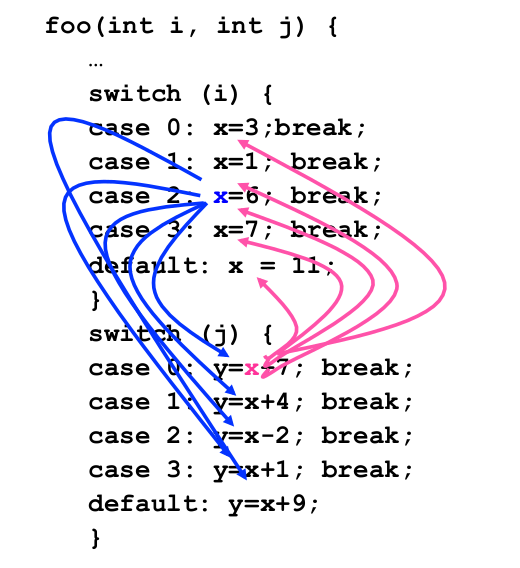
\includegraphics[width=0.3\textwidth]{p38.png}
    \caption{If a variable has N uses and M definitions (which occupy about N + M instructions in a program), it takes space (and time) proportional to N · M to represent def-use chains – a quadratic blowup.}
    \label{fig:p38}
\end{figure}


\subsection{Static Single Assignment(SSA)}

\begin{definition}{Static Single Assignment }
    Static Single Assignment is an IR where every variable is assigned a value at most once in the program text.
\end{definition}








\begin{definition}{the $\Phi$ function}

     $\Phi$ merges multiple definitions along multiple control paths into a single definition.

     At a basic block with p predecessors, there are p arguments to the $\Phi$ functions.

     $$ x_{\text {new }} \leftarrow \Phi\left(\mathbf{x}_1, \mathbf{x}_1, \mathbf{x}_1, \ldots, \mathbf{x}_{\mathrm{p}}\right)
     $$
\end{definition}

\subsubsection{Why SSA is useful?}

\textbf{ \large \textit{Useful for Dataflow Analysis}} Dataflow analysis and optimization algorithms can be made simpler when each variable has only one definition.

\textbf{ \large \textit{Less space and time complexity}} If a variable has N uses and M definitions (which occupy about N + M instructions in a program), it takes space (and time) proportional to N · M to represent def-use chains – a quadratic blowup. For almost all realistic programs, the size of the SSA form is linear in the size of the original program.


\textbf{ \large \textit{Simplify some algorithms}} Uses and defs of variables in SSA form relate in a useful way to the dominator structure of the control-flow graph, which simplifies algorithms such as interference-graph construction.


\textbf{ \large \textit{Eliminate needless relationship}} Unrelated uses of the same variable in the source program become different variables in SSA form, eliminating needless relationships shown in \ref{exp:1}.

\begin{lstlisting}[label={exp:1},caption={An example}]

for i <- 1 to N do A[i] <- 0
for i <- 1 to M do s <- s + B[i]

\end{lstlisting}


\subsection{How to represent SSA?}

In straight-line code, such as within a basic block, it is easy to see that each instruction can define a fresh new variable instead of redefining an old one shown in \ref{fig:p42-43}


\begin{figure}[htb]
     \centering
     \begin{subfigure}{0.2\textwidth}
     \centering
         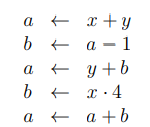
\includegraphics[width=\textwidth]{p42.png}
         \caption{A straight-line program.}
         \label{fig:p42}
     \end{subfigure}
     \begin{subfigure}{0.25\textwidth}
     \centering
         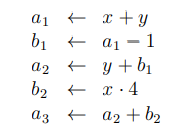
\includegraphics[width=\textwidth]{p43.png}
         \caption{The program in single-assignment form.}
         \label{fig:p43}
     \end{subfigure}
        \caption{SSA for straight-line code}
        \label{fig:p42-43}
\end{figure}


But when two control-flow paths merge together, it is not obvious how to have only one assignment for each variable. To solve this problem we introduce a notational fiction, called a $\Phi$ function. Figure \ref{fig:p44} shows that we can combine a1 (defined in block 1) and a2 (defined in block 3) using the function $a3 \leftarrow \Phi(a1, a2)$.


\begin{figure}[htb]
    \centering
    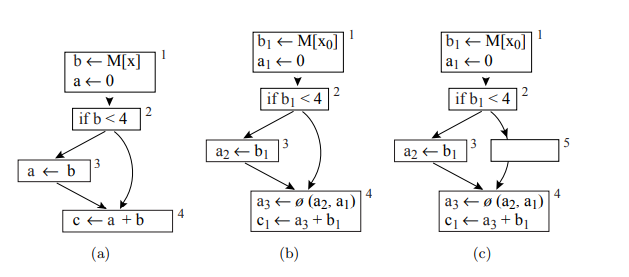
\includegraphics[width=0.8\textwidth]{p44.png}
    \caption{(a) A program with a control-flow join; (b) the program transformed to single-assignment form; (c) edge-split SSA form.}
    \label{fig:p44}
\end{figure}


unlike ordinary mathematical functions, $\Phi$(a1, a2) yields a1 if control reaches block 4 along the edge $2 \rightarrow 4$, and yields a2 if control comes in on edge $3 \rightarrow 4$.


\subsubsection{How does the $\phi$-function know which edge was taken?}


If we must execute the program, or translate it to executable form, we can “implement” the $\Phi$-function using a move instruction on each incoming edge as shown in Figure \ref{fig:p39-40}. However, in many cases, we simply need the connection of uses to definitions and don’t need to “execute” the $\Phi$-functions during optimization. In these cases, we can ignore the question of which value to produce.

\begin{figure}[htb]
     \centering
     \begin{subfigure}{0.3\textwidth}
     \centering
         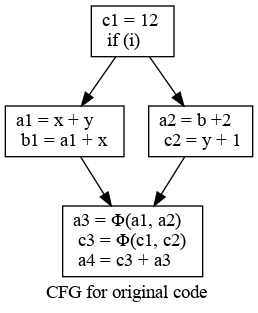
\includegraphics[width=\textwidth]{p39.png}
         \caption{Original code}
         \label{fig:p39}
     \end{subfigure}
     \begin{subfigure}{0.3\textwidth}
     \centering
         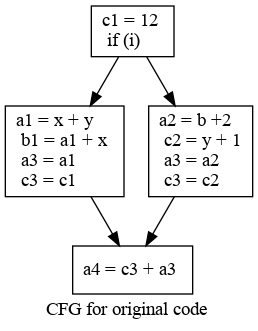
\includegraphics[width=\textwidth]{p40.png}
         \caption{Code after moving instruction.}
         \label{fig:p40}
     \end{subfigure}
        \caption{Implementing $\Phi$-function}
        \label{fig:p39-40}
\end{figure}




\subsection{Converting to SSA form}

The algorithm for converting a program to SSA form is roughly as follows:

\begin{itemize}
    \item 1. adds $\Phi$ functions for the variables, and then
    \item 2. renames all the definitions and uses of variables using subscripts.
\end{itemize}




\subsubsection{Trivial SSA}

Trivial SSA form is based on a simple observation: $\Phi$ functions are only needed for variables that are "live" after the $\Phi$ function.

\begin{itemize}
    \item Each assignment generates a fresh variable.
    \item At each join point insert $\Phi$ for all live variables.
\end{itemize}


Trivial SSA will generate some useless $\Phi$ functions. An example is shown in Figure \ref{fig:p41} So a $\Phi$-function is not needed for every variable at each point.

\begin{figure}[htb]
    \centering
    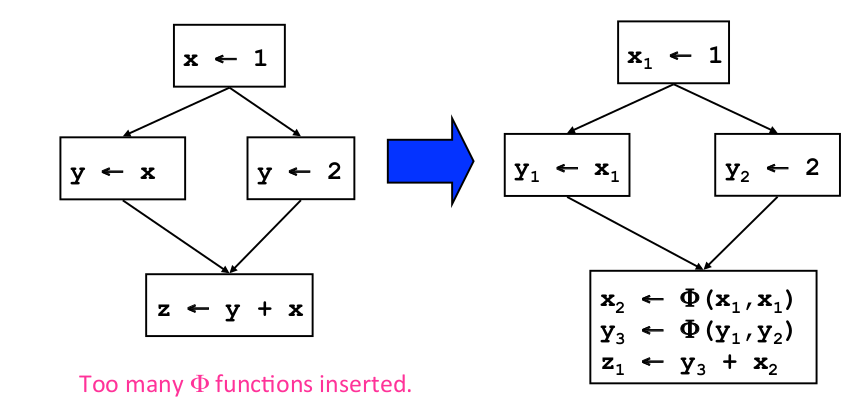
\includegraphics[width=0.5\textwidth]{p41.png}
    \caption{$x2 \leftarrow \Phi(x1,x1)$ is useless because x2 is equal to x1.}
    \label{fig:p41}

\end{figure}



\subsubsection{Minimal SSA}
Minimal SSA is an updated version compared to trivial SSA.

\begin{itemize}
    \item Each assignment generates a fresh variable.
    \item At each join point insert $\Phi$ for all live variables with multiple outstanding defs. 
\end{itemize}

\subsubsection{Path-convergence criterion}

There should be a $\Phi$-function for variable a at node z of the flow graph
exactly when all of the following are true:

\begin{itemize}
    \item 1. There is a block x containing a definition of a,
    \item 2. There is a block y (with $y \neq x$) containing a definition of a,
    \item 3. There is a nonempty path $P_{xz}$ of edges from x to z,
    \item 4. There is a nonempty path $P_{yz}$ of edges from y to z,
    \item 5. Paths $P_{xz}$ and $P_{yz}$ do not have any node in common other than z, and
    \item 6. The node z does not appear within both $P_{xz}$ and $P_{yz}$ prior to the
end, though it may appear in one or the other.
\end{itemize}


We consider the start node to contain an implicit definition of every variable, either because the variable may be a formal parameter or to represent the notion of a 
$\leftarrow$ uninitialized without special cases. A $\Phi$-function itself counts as a definition of a, so the path-convergence criterion must be considered as a set of equations to be satisfied. As usual, we can solve them by iteration as shown in \ref{alg:Iterated path-convergence criterion}.


\begin{algorithm}
\caption{Iterated path-convergence criterion}\label{alg:Iterated path-convergence criterion}
\begin{algorithmic}

\While{there are nodes $x, y, z$ satisfying conditions 1–5
and \\ $z$ does not contain a $\Phi$-function for a}
\State  insert a $\leftarrow$ $\Phi$(a, a, . . . , a) at node Z
\EndWhile
\end{algorithmic}
\end{algorithm}

\subsubsection{Dominance property of SSA form}

The iterated path-convergence algorithm for placing $\Phi$-functions is not practical, since it would be very costly to examine every triple of nodes x, y, z, and every path leading from x and y.  A much more efficient algorithm using the dominator tree of the flow graph as shown in Figure \ref{fig:p45}.


\begin{figure}[H]
    \centering
    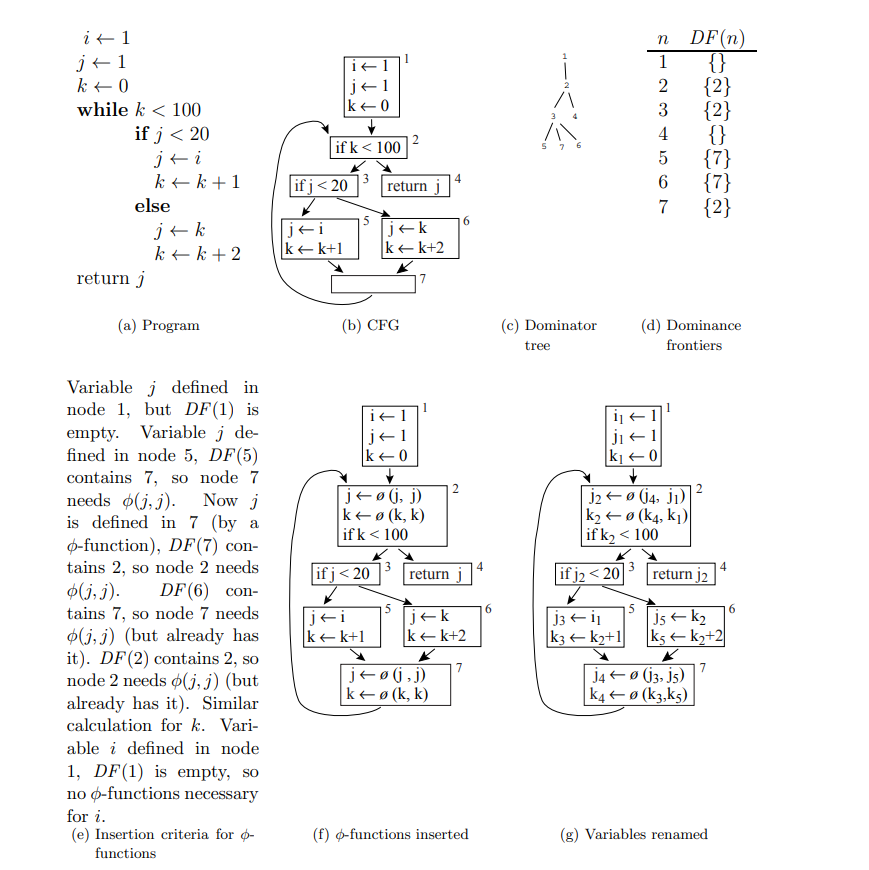
\includegraphics[width=\textwidth]{p45.png}
    \caption{ Conversion of a program to static single-assignment form. Node 7 is a postbody node, inserted to make sure there is only one loop edge; such nodes are not strictly necessary but are sometimes helpful.}
    \label{fig:p45}

\end{figure}


\begin{definition}{Strictly dominance}
    x strictly dominates w (x sdom w) iff impossible to reach w without passing through x first.
\end{definition}

\begin{definition}{Dominance}
    x  dominates w (x dom w) iff x sdom w or x = w.
$$
\operatorname{Dom}(n)= \begin{cases}\{n\} & \text { if } n=n_0 \\ \{n\} \cup\left(\bigcap_{p \in \operatorname{preds}(n)} \operatorname{Dom}(p)\right) & \text { if } n \neq n_0\end{cases}
$$
\end{definition}

\begin{definition}{Dominance tree}
    x sdom w iff x is a proper ancestor of w.  

\end{definition}

\begin{definition}{Dominance Frontier}


The dominance frontier of a node x is the set of all nodes w such that
x dominates a predecessor of w, but does not strictly dominate w.

$$
F(x)=  \{w | \texttt{x  dom pred(w) AND   !(x  sdom  w) } \}
$$
\end{definition}





An essential property of static single assignment form is that definitions dominate uses; more specifically,
\begin{itemize}
    \item  If x is the ith argument of a $\Phi$-function in block n, then the definition of x dominates the ith predecessor of n.
    \item  If x is used in a non-$\Phi$ statement in block n, then the definition of x dominates n
\end{itemize}

\begin{note}{Dominance Property of SSA	}
  In SSA,

  \begin{itemize}
      \item If x i is used in $x \leftarrow \Phi (..., x_i , ...)$, then $BB(x_i )$ dominates ith predecessor of $BB(\Phi)$
      \item If x is used in $y \leftarrow ...x...$,then BB(x) dominates BB(y)
  \end{itemize}
\end{note}


\textbf{ \large \textit{Dominance frontier criterion.}} Whenever node x contains a definition of some variable a, then any node z in the dominance frontier of x needs a $\Phi$-function for a.


\textbf{ \large \textit{Iterated dominance frontier.}} Since a $\Phi$-function itself is a kind of definition, we must iterate the dominance-frontier criterion until there are no nodes that need $\Phi$-functions.


\textbf{ \large \textit{Theorem.}} The iterated dominance frontier criterion and the iterated path convergence criterion specify exactly the same set of nodes at which to put $\Phi$-functions

\begin{figure}[htb]
    \centering
    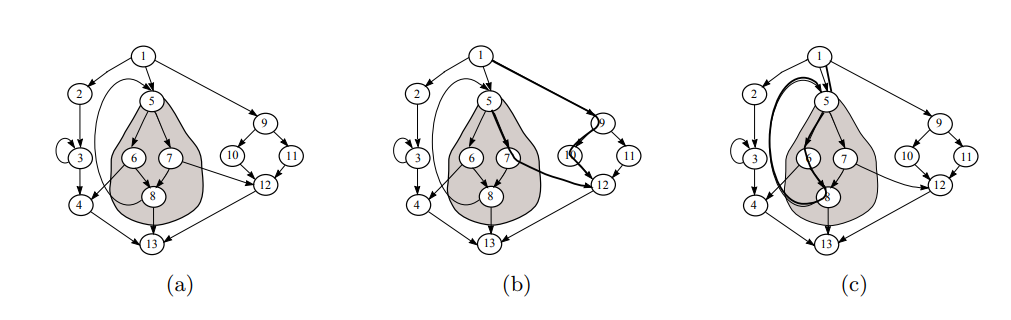
\includegraphics[width=\textwidth]{p46.png}
    \caption{Node 5 dominates all the nodes in the grey area. (a) Dominance frontier of node 5 includes the nodes (4, 5, 12, 13) that are targets of edges crossing from the region dominated by 5 (grey area including node 5) to the region not strictly dominated by 5 (white area including node 5). (b) Any node in the dominance frontier of n is also a point of convergence of nonintersecting paths, one from n and one from the root node. (c) Another example of converging paths $P_{1,5}$ and $P_{5,5}$.}
    \label{fig:p46}

\end{figure}


\begin{proof}{Proof}
The sketch of a proof that shows if w is in the dominance frontier of a definition, then it must be a point of convergence.

Suppose there is a definition of variable a at some node n (such as node 5 in Figure  \ref{fig:p46}b), and node w (such as node 12 in Figure  \ref{fig:p46}b) is in the dominance frontier of n. The root node implicitly contains a definition of every variable, including a. There is a path $P_{rw}$ from the root node (node 1 in Figure \ref{fig:p46}) to w that does not go through n or through any node that n dominates; and there is a path $P_{nw}$ from n to w that goes only through dominated nodes. These paths have w as their first point of convergence.
\end{proof}


\subsection{Computing the dominance frontier}

To insert all the necessary $\Phi$-functions, for every node n in the flow graph we need DF[n], its dominance frontier. Given the dominator tree, we can efficiently compute the dominance frontiers of all the nodes of the flow graph in one pass. We define two auxiliary sets

\begin{itemize}
    \item $DF_{local}[n]$ The successors of n that are not strictly dominated by n;
    \item $DF_{up}[n]$ Nodes in the dominance frontier of n that are not dominated by n’s immediate dominator.
\end{itemize}

The dominance frontier of n can be computed from $DF_{local}[n]$  and $DF_{up}[n]$ 


$$
D F[n]=D F_{\text {local }}[n] \quad \cup \quad \bigcup_{c \in \text { children }[n]} D F_{\text {up }}[c]
$$

where children[n] are the nodes whose immediate dominator (idom) is n.


To compute $DF_{local}[n]$ \ref{alg:computeDF} more easily (using immediate dominators instead of dominators), we use the following theorem: $DF_{local}[n]$ = the set of those successors of n whose immediate dominator is not n. The following computeDF function should be called on the root of the dominator tree (the start node of the flow graph). It walks the tree computing DF[n] for every node n: it computes $DF_{local}[n]$ by examining the successors of n, then combines $DF_{local}[n]$ and (for each child c) $DF_{up}[n]$.a

\begin{algorithm}
\caption{computeDF}\label{alg:computeDF}
\begin{algorithmic}

\State $S \gets \{\}$
\For{each node y in succ[n]} \Comment{This loop computes $DF_{local}[n]$}
\If {idom(y) $\neq$ n}
\State $S\leftarrow S \cup \{y\}$
\EndIf 
\EndFor

\For{each child c of n in the dominator tree} 
\State computeDF[c]
\For{each element w of DF[c]} \Comment{This loop computes $DF_{up}[n]$}
\If {n does not dominate w}
\State $S\leftarrow S \cup \{w\}$
\EndIf 
\EndFor
\EndFor
\end{algorithmic}
\end{algorithm}

This algorithm is quite efficient. It does work proportional to the size (number of edges) of the original graph, plus the size of the dominance frontiers it computes. Although there are pathological graphs in which most of the nodes have very large dominance frontiers, in most cases the total size of all the DFs is approximately linear in the size of the graph, so this algorithm runs in “practically” linear time.




\subsection{Inserting $\Phi$-functions}

Starting with a program not in SSA form, we need to insert just enough $\Phi$-functions to satisfy the iterated dominance frontier criterion. To avoid re-examining nodes where no $\Phi$-function has been inserted, we use a work-list algorithm.

\begin{algorithm}
\caption{Place-$\Phi$-Functions}\label{alg:Place-Phi-Functions}
\begin{algorithmic}
\For{each node n}
\For{each variable a in $A_{orig}[n]$}
\State defsites[a] $\gets$ defsites[a] $\cup \{n\}$
\EndFor
\EndFor


\For{each variable a}
\State W $\gets$ defsites[a]
\While{ W not empty}
\State{remove some node n from W}
\For{each y in DF[n]}
\If{y $\not\in$ $A_{\Phi}[a]$}
\State{insert the statement a $\gets$ $\Phi$(a, a, . . . , a) at the top of block y, where the $\Phi$-function has as many arguments as y has predecessors}
\State{$A_{\Phi}[a] \gets A_{\Phi}[a] \cup \{ y\}$}
\If{a $\not\in$ $A_{orig}[y]$}
\State{$W \gets W \cup \{y \}$}
\EndIf

\EndIf
\EndFor
\EndWhile
\EndFor

\end{algorithmic}
\end{algorithm}


Algorithm\ref{alg:Place-Phi-Functions} starts with a set V of variables, a graph G of controlflow nodes – each node is a basic block of statements – and for each node n a set $A_{orig}$[n] of variables defined in node n. The algorithm
computes $A_{\Phi}[a]$, the set of nodes that must have $\Phi$-functions for variable
a. Sometimes a node may contain both an ordinary definition and a
$\Phi$-function for the same variable; for example, in Figure \ref{fig:p46}b, a $\in$ $A_{orig}[2]$
and 2 $\in$ $A_{\Phi}[a]$.


This algorithm does a constant amount of work (a) for each node and edge in the control-flow graph, (b) for each statement in the program, (c) for each element of every dominance frontier, and (d) for each inserted $\Phi$-function. For a program of size N, the amounts a and b are proportional to N, c is usually approximately linear in N. The number of inserted $\Phi$-functions (d) could be $N^2$ in the worst case, but empirical measurement has shown that it is usually proportional to N. So in practice, Algorithm \ref{alg:Place-Phi-Functions} runs in approximately linear time.


\subsection{Renaming the variables}

After the $\Phi$-functions are placed, we can walk the dominator tree, renaming the different definitions (including $\Phi$-functions) of variable a to a1, a2, a3 and so on. Rename each use of a to use the closest definition d of a that is above a in the dominator tree. Algorithm  renames all uses and definitions of variables, after the $\Phi$-functions have been inserted by Algorithm \ref{alg:Renaming variables}. In traversing the dominator tree, the algorithm “remembers” for each variable the most recently defined version of each variable, on a separate stack for each variable. Although the algorithm follows the structure of the dominator tree – not the flow graph – at each node in the tree it examines all outgoing flow edges, to see if there are any $\Phi$-functions whose operands need to be properly numbered.



\begin{algorithm}
\caption{Renaming variables.}\label{alg:Renaming variables}
\begin{algorithmic}
\State Initialization:

\For{each variable a}
\State{Count[a] $\gets$ 0}
\State{Stack[a] $\gets$ empty}
\State{push 0 onto Stack[a]}
\EndFor

\State{Rename(n) }
\For{each statement S in block n}
\If{S is not a $\Phi$-function}
\For{each use of some variable x in S}
\State{i $\gets$ top(Stack[x])}
\State{replace the use of x with $x_i$ in S}
\EndFor
\EndIf
\For{each definition of some variable a in S}

\State Count[a] $\gets$ Count[a]+1
\State i $\gets$ Count[a]
\State push i onto Stack[a]
\State replace definition of a with definition of $a_i$ in S
\EndFor
\EndFor

\For{each successor Y of block n,}
\State Suppose n is the jth predecessor of Y
\For{each $\Phi$-function in Y}
\State suppose the jth operand of the $\Phi$-function is a
\State i $\gets$ top(Stack[a])
\State replace the jth operand with $a_i$

\EndFor
\EndFor
\For{each child X of n}
\State Rename(X)
\EndFor
\For{each definition of some variable a in the original S}
\State pop Stack[a]
\EndFor
\end{algorithmic}
\end{algorithm}




\subsection{Edge Splitting}

Some analyses and transformations including reverse transformation from SSA back into a normal form are simpler if there is never a controlflow edge that leads from a node with multiple successors to a node with multiple predecessors. To give the graph this unique successor or predecessor property, we perform the following transformation: For each control-flow edge a $\gets$ b such that a has more than one successor and b has more than one predecessor, we create a new, empty controlflow node z, and replace the a $\gets$ b edge with an a $\gets$ z edge and a z $\gets$ b edge.

An SSA graph with this property is in edge-split SSA form. Figure \ref{fig:p44} illustrates edge splitting. Edge splitting may be done before or after insertion of $\Phi$-functions.
\newpage

\section{SSA-Style optimizations}

\subsection{Constant Propagation}
\begin{note}{notes}
\begin{itemize}
    \item If  v $\gets$ c , replace all uses of v with c 
    \item If  v $\gets$  $\Phi$ (c,c,c)  (each input is the same constant), replace all uses of v with c
\end{itemize}
\end{note}


\begin{algorithm}
\caption{SSA-CP}\label{alg:SSA-CP}
\begin{algorithmic}
\State{W $\gets$ ist of all defs}
\While{!W.isEmpty}

\State{Stmt S $\gets$ W.removeOne}
\If{(S has form v $\gets$ c) or
(S has form v $\gets$ $\Phi$(c,...,c))}
\State delete S
\For{each stmt U that uses v}
\State {replace v with c in U}
\State {W.add(U)}
\EndFor
\EndIf
\EndWhile

\end{algorithmic}
\end{algorithm}

\subsection{Conditional Constant Propagation }

Wegman and Zadeck's Sparse Conditional Constant (SCC) algorithm was used to find constant expressions, constant conditions, and unreachable code [WZ91]. The output of the SCC algorithm is an association of variables to one of $\lbrace \bot, c, \top \rbrace$, where $\bot$ marks a variable that can hold different values at different times, and $\top$ means the variable is not executed. In addition, every flow-graph node (corresponding to a quadruple) is marked as executable or non-executable. We then walk the flow-graph, eliminating dead-code (quadruples marked non-executable), replacing constant variables with their values, and changing constant conditional branches to goto statements.

\begin{note}{notes}
\begin{itemize}
    \item Assume all blocks unexecuted until proven otherwise
    \item Assume all variables are not executed (only with proof of assignment of a non-constant value do we assume not constant)
\end{itemize}
\end{note}

\subsubsection{Example}

\begin{figure}[H]
    \centering
     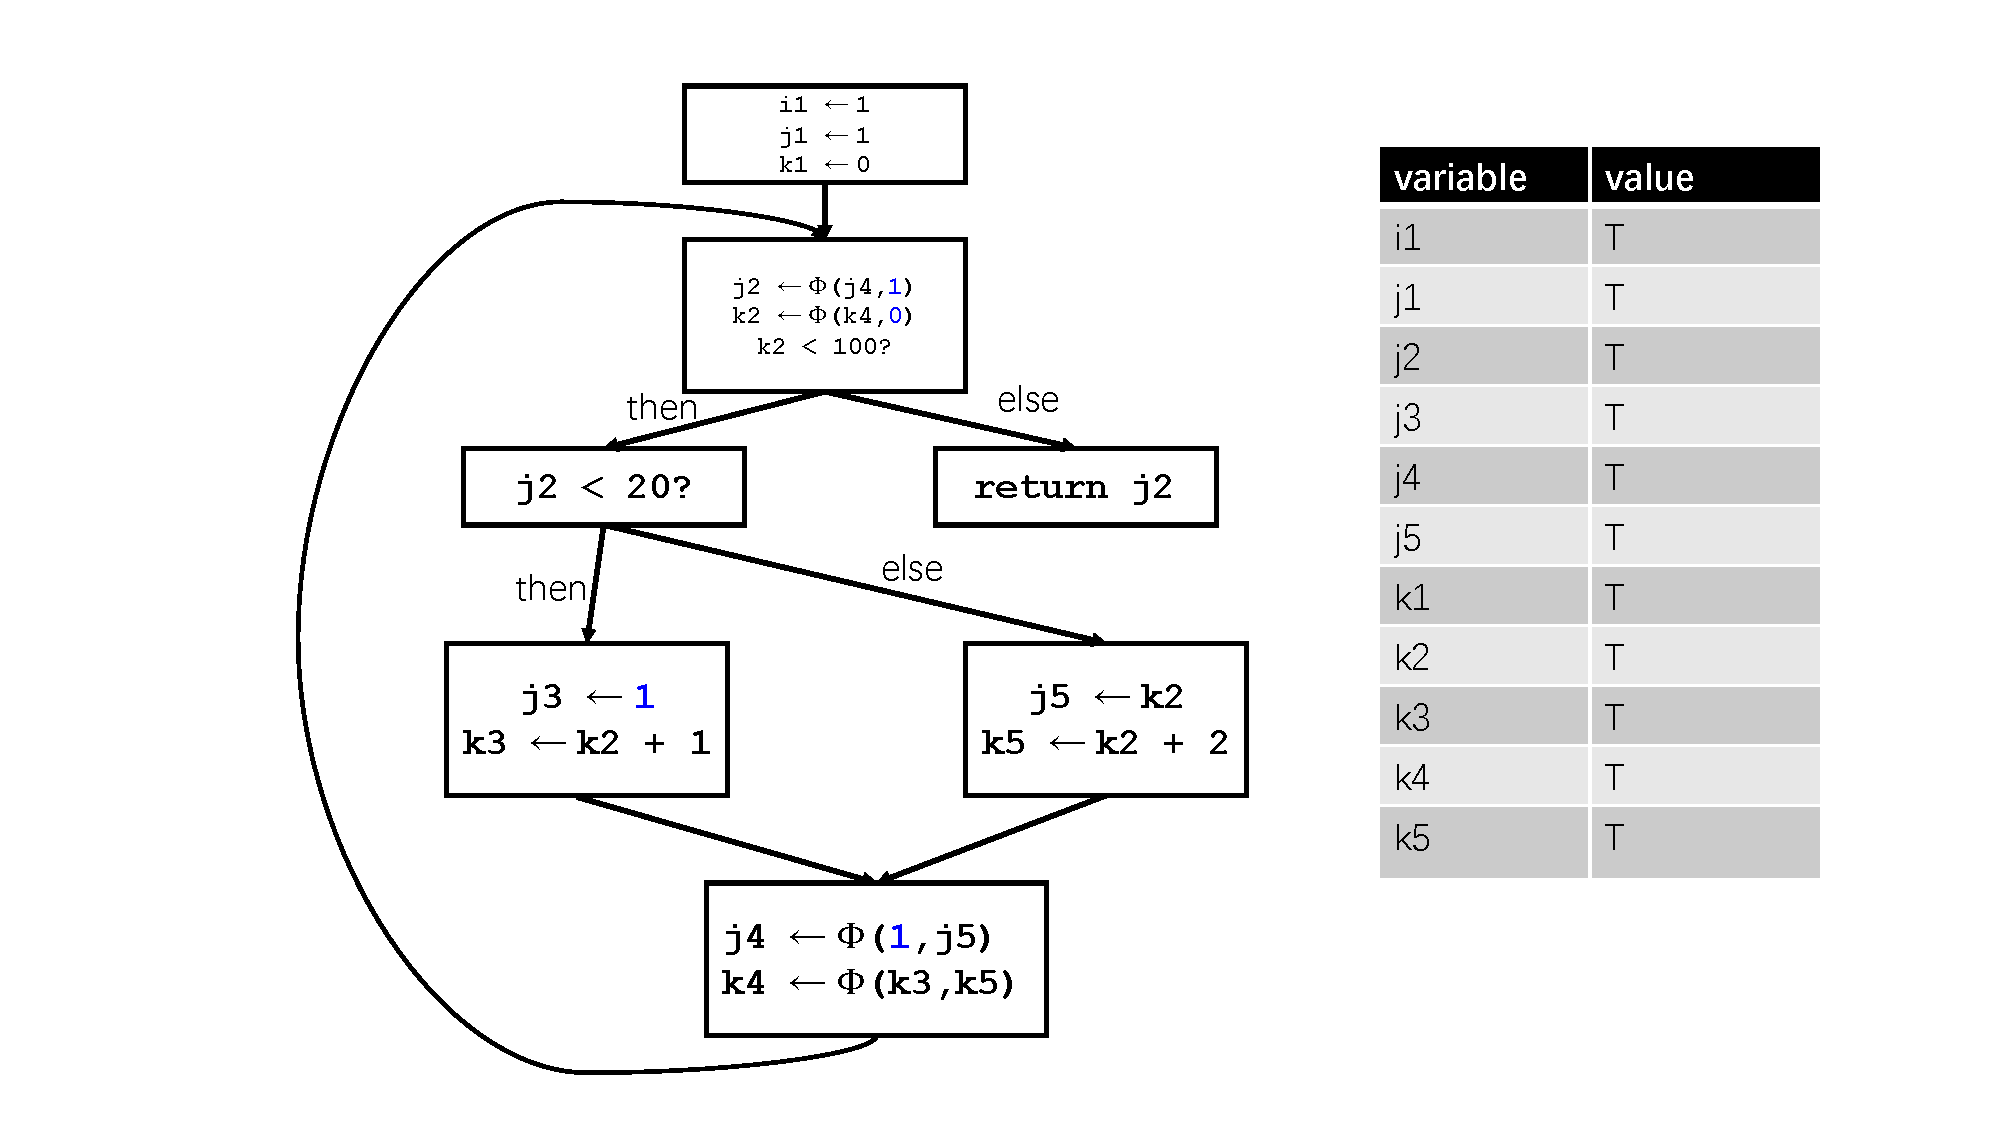
\includegraphics[width=\textwidth]{p47.pdf}
         \caption{Original code. The black block is marked as unexecuted}
         \label{fig:p47}

\end{figure}




\begin{figure}[H]
    \centering
     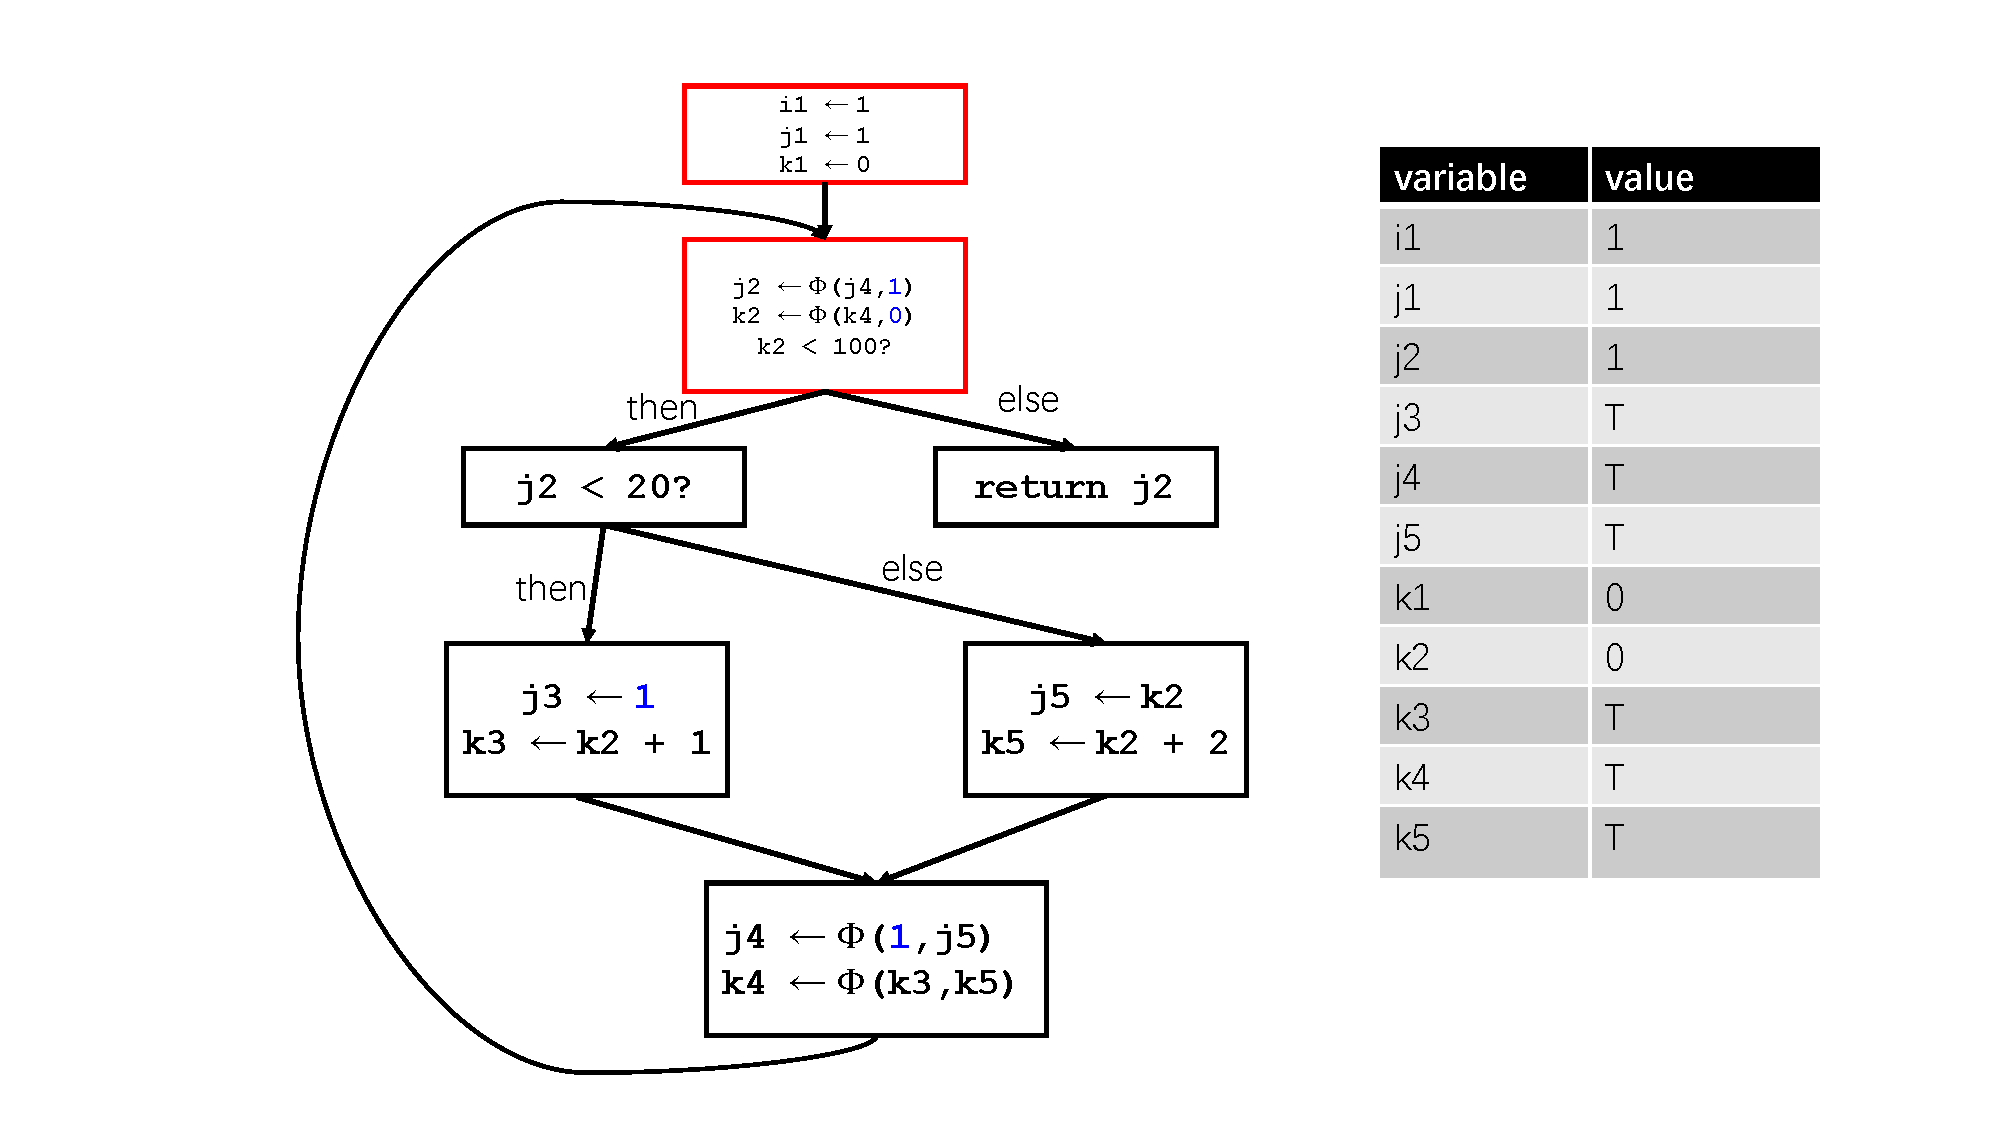
\includegraphics[width=0.8\textwidth]{p48.pdf}
         \caption{The read block is marked as executed. After walking the first two blocks, the value is shown above.}
         \label{fig:p48}

\end{figure}



\begin{figure}[H]
    \centering
     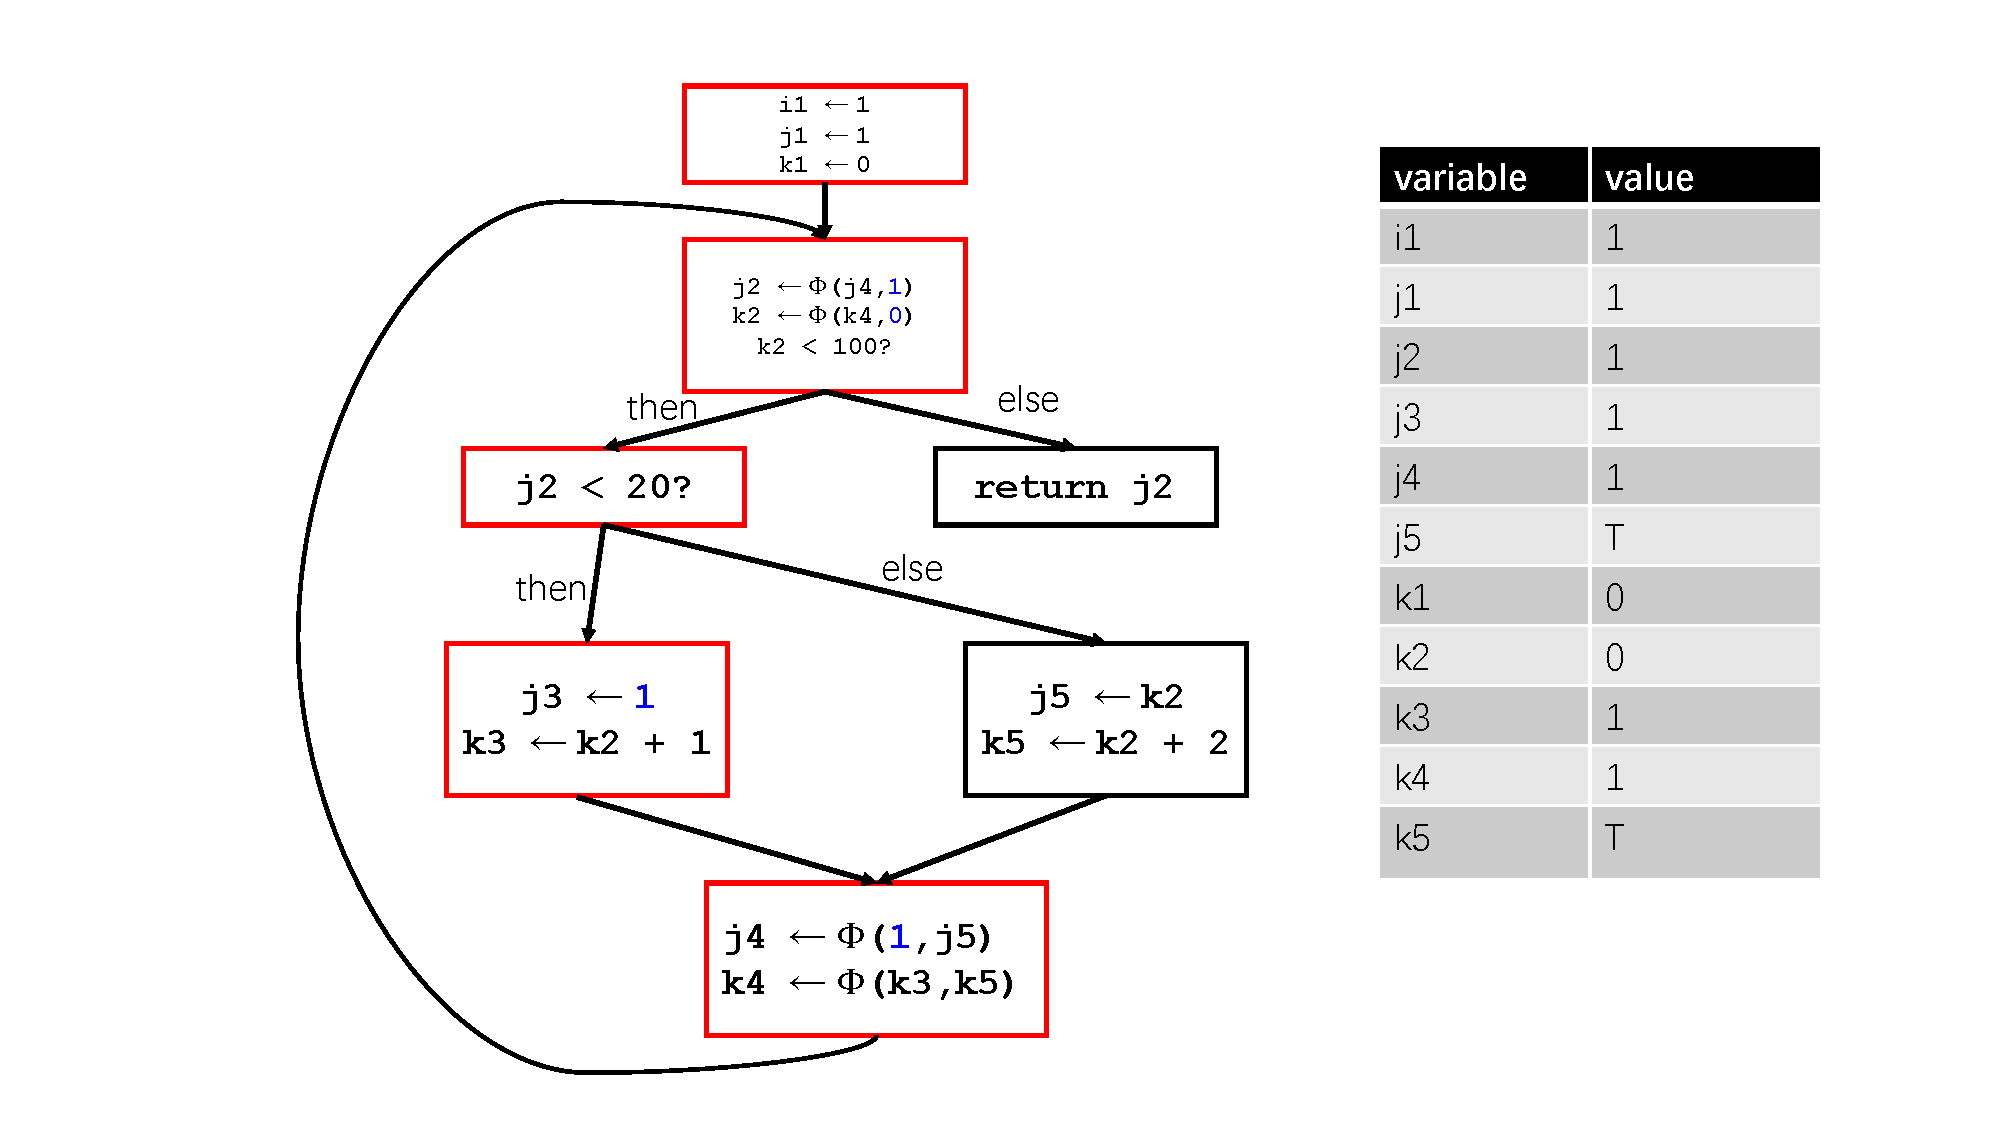
\includegraphics[width=0.8\textwidth]{p49.pdf}
         \caption{After walking 5 blocks.}
         \label{fig:p49}

\end{figure}



\begin{figure}[H]
    \centering
     \includegraphics[width=0.8\textwidth]{p50.pdf}
         \caption{Now k2 is $\bot$, so the \texttt{return j2} is reachable.}
         \label{fig:p50}

\end{figure}



\begin{figure}[H]
    \centering
     \includegraphics[width=0.5\textwidth]{p51.pdf}
         \caption{Code after applied SCC.}
         \label{fig:p51}

\end{figure}


% \begin{figure}[!b]
%      \centering
%      \begin{subfigure}{0.45\textwidth}
%      \centering
%          \includegraphics[width=\textwidth]{p47.pdf}
%          \caption{Original code}
%          \label{fig:p47}
%      \end{subfigure}
%      \begin{subfigure}{0.6\textwidth}
%      \centering
%          \includegraphics[width=\textwidth]{p48.pdf}
%          \caption{Code after moving instruction.}
%          \label{fig:p48}
%      \end{subfigure}
%           \begin{subfigure}{0.6\textwidth}
%      \centering
%          \includegraphics[width=\textwidth]{p49.pdf}
%          \caption{Code after moving instruction.}
%          \label{fig:p49}
%      \end{subfigure}
%           \begin{subfigure}{0.6\textwidth}
%      \centering
%          \includegraphics[width=\textwidth]{p50.pdf}
%          \caption{Code after moving instruction.}
%          \label{fig:p50}
%      \end{subfigure}
%           \begin{subfigure}{0.6\textwidth}
%      \centering
%          \includegraphics[width=\textwidth]{p51.pdf}
%          \caption{Code after moving instruction.}
%          \label{fig:p51}
%      \end{subfigure}
%         \caption{Implementing $\Phi$-function}
%         \label{fig:p47-51}
% \end{figure}




\subsection{Copy Propogation}

\begin{note}{notes}
\begin{itemize}
    \item  delete x $\gets \Phi$ (y,y,y) and replace all x with y
    \item delete x $\gets$ y and replace all x with y
\end{itemize}
\end{note}









\printbibliography

\end{document}
